\documentclass[12pt]{article}

\usepackage{graphicx}
\usepackage{pdfpages}
\usepackage{listings}
\usepackage{amsmath}
\usepackage{subcaption}
\usepackage{todonotes}
\usepackage{arydshln}

\renewcommand{\figurename}{Fig.}

\title{TTK4210 Advanced Control of Industrial Systems, Exercise 6}
\date{}
\author{Kristian Løvland}

\begin{document}
\maketitle
\newpage
\tableofcontents

\newpage
\section{Abstract}
In this project, a model of a butane distillation column was used to design a controller for the composition of two product streams consisting of n-butane and iso-butane, respectively. By identifying characteristics of relevant subsystems, PI controllers for the states of these systems were designed with the ultimate goal of keeping the purity of the products at a satisfactory level. In the end, quick control without excessive oscillation was acheived.

\newpage
\section{Introduction}

\subsection{Structure of the report}
The system analysis, controller design, controller tuning and results are presented in the order they were done. All experiments referred to when doing system identification are plotted in the appendix to avoid drowning the reader in plots. Matlab code is included where it was considered necessary.

\subsection{Problem summary}
A good introduction to the control problem we're faced with is given in the assignment text \cite{oppgavetekst}. A short summary follows.

The top product is required to contain no more than 4\% n-butane, while the bottom product is required to contain less than 2,5\% iso-butane. 

These compositions, denoted $x_D^*$ and $x_B^*$, are in practice controlled through their temperatures. These are measured on the top and bottom of the distillation column, and are denoted $T_D$ and $T_B$. The temperature needed to acheive the required compositions are shown in table \ref{tab:requirements}, together with the actual temperature setpoint. These are a bit lower/higher than than strictly necessary to introduce a safety margin.

\begin{table}[h]
\centering
\begin{tabular}{c | c | c }
& Required temperature & Temperature setpoint\\ \hline
Top product ($D$) & $35,85^\circ$ C & $35,30^\circ$ C\\
Bottom product ($B$) & $47,69^\circ$ C & $48,51^\circ$ C
\end{tabular}
\caption{Temperatures giving satisfactory product quality}
\label{tab:requirements}
\end{table}

To satisfy these specifications, the rest of the states in the system need to stay in reasonable areas. This means levels $M_D$ in the top accumulator and $M_B$ in the distillation column, together with distillation column pressure $p$, need to be controlled stably to their setpoints.

To control these five variables, five degrees of freedom is needed. Our five manipulated variables are flow rates in different parts of the system, denoted $V_T$, $L$, $D$, $V$ and $B$. Each of these are controlled by their own inputs, mostly valves.

Table \ref{tab:pairings} shows the pairing of manipulated and controlled variables. As mentioned, it is assumed that choosing good setpoints for $T_D$ and $T_B$ gives satisfactory product quality. This control structure is called LV-control, after the manipulated variables used to control product quality.

\begin{table}[h]
\centering
\begin{tabular}{c|ccccc}
Manipulated Variable & $V_T$ & $D$ & $B$ & $L$ & $V$ \\ \hline
Controlled variable & $p$ & $M_D$ & $M_B$ & $T_D$ & $T_B$
\end{tabular}

\caption{Variable pairings}
\label{tab:pairings}
\end{table}

\newpage
\section{Secondary controllers}
The secondary controllers were tuned individually using the SIMC method for PI controllers. A step in process input of $50\%$ of maximum input was used for all the secondary controllers controlling the states $D$, $L$, $B$ and $p$. For $V$, a step input change of $20\%$ was used to avoid effects from other parts of the system.

\subsection{The SIMC method}
A summary of the SIMC method is given in \cite{regtek}. The method assumes that the system can be approximated by a first order process with time delay, which has transfer function

\begin{equation}
G(s) = \frac{k e^{-\theta s}}{1 + T_1 s}
\end{equation}
This system is to be controlled by a PI controller

\begin{equation}
K(s) = K_p\frac{1 + T_i s}{T_i s}
\end{equation}

The SIMC method gives rules for choosing $K_p$ and $T_i$, given a desired closed-loop time contant $T_L$. The two steps of the method are then

\begin{enumerate}
\item Fit the step response to a first order model. This means finding time delay $\theta$, slope $k' = \frac{dy/dt}{\Delta u}$ and time constant $T_1$ from the plot of the step response.
\item To achieve the desired time constant $T_L$, use the PI controller parameters $K_p = \frac{1}{k'} \frac{1}{\tau + T_L}$, $T_i = \min(T_1, 4(\tau + T_L))$.
\end{enumerate}
How one chooses $T_L$ depends on the desired response. In \cite{regtek}, $T_L = 0.3\tau$ is suggested for "aggressive" control. If no overshoot is desired, one should choose $T_L > 2 \tau$.

\subsection{Tuning}
The step experiments can be seen in figures \ref{fig:ol_step_FC1005}, \ref{fig:ol_step_FC1015}, \ref{fig:ol_step_FC1019}, \ref{fig:ol_step_LC1028} and \ref{fig:ol_step_PC1024}. The reference signals should have been omitted from these plots since we are dealing with open loop systems, and can safely be ignored here.

The plots show that for the first three variables, the accuracy of the simulation is clearly not sufficient for fitting a first order model (they behave in a stepwise fashion). Inspecting the orders of magnitude of the gains and time constants may however still be useful. To approximate their sizes, a straight line was drawn from initial state to steady-state. Its slope was considered to be $\frac{dy}{dt}$, and the point where this line crossed $63\%$ of the change was considered to be the time constant. This method clearly causes underestimates of $\frac{dy}{dt}$ and overestimates of $T_1$, but it's hard to find a meaningful way to fit a tangent given the insufficient information. For the two other variables, more reasonable readings could be done. All results are shown in table \ref{tab:inner_loop_step_responses}.

Our desired time constant $T_L$ for each loop is shown in the table as well. Initially, $T_L = 0,3\tau$ was chosen for the three fastest loops. Some simple trial and error in K-spice showed that this lead to oscillation and unfortunate interaction between control loops, especially the controllers for $D$ and $L$. This is probably partly due to the underestimates of $k'$ and $T_1$ for these variables. Conservative estimates of these results in more aggressive controllers (to compensate for the slow system) when using the SIMC method.

Due to this unsatisfactory behaviour, $T_L = 2\tau$ was chosen for the three fastest control loops instead. The time delay was hard to make a meaningful reading of for the two other systems, so a somewhat arbitrary choice of $T_L = 10s$ was chosen for these systems (instead of using the $T_L = 2\tau$ rule). Like all the other parameters, these were not absolute choices, but a good starting point for further tuning.

After calculating the SIMC controller values, some more qualitative tuning using K-spice simulations was not surprisingly needed. For $D$ and $L$, the integral times were kept fixed, while the gain needed to be decreased to avoid oscillations. For $B$, it was necessary to reduce the integral time in addition to reducing the gain to avoid oscillation. The response of $V$ was slow, and to avoid bandwith limitations in the control of $T_B$ later, both controller parameters were changed to give dramatically more aggressive behaviour. For $p$, the stationary deviation was initially removed pretty slowly, so the integral time was reduced, while also reducing gain to avoid oscillation.

The results of implementing these controllers in K-spice, using the internally scaled gain $G = K_p \frac{(y_{\max} - y_{\min})}{(u_{\max} - u_{\min})}$ for all controllers, are shown in figures \ref{fig:cl_step_FC1005}, \ref{fig:cl_step_FC1015}, \ref{fig:cl_step_FC1019}, \ref{fig:cl_step_LC1028} and \ref{fig:cl_step_PC1024}.

\begin{table}
\centering
\begin{tabular}{c | c | c | c | c | c || c}
& $\tau$ & $T_1$ & $\frac{dy}{dt}$ & $\Delta u$ & $k'$ & $T_L$ \\ \hline
$D$ & 1,0s & 0,4s & 14,3 & 50\% & 28,6 & 2s \\
$L$ & 1,0s & 1,0s & 47,5 & 50\% & 95,0 & 2s \\
$B$ & 1,0s & 0,6s & 10,0 & 50\% & 20,0 & 2s \\
$V$ & $\approx$ 0 & 400s & 0,028 & 20\% & 0,14 & 10s \\
$p$ & $\approx$ 0 & 200s & 0,088 & 50\% & 0,18 & 10s
\end{tabular}
\caption{Identified parameters for inner loop}
\label{tab:inner_loop_step_responses}
\end{table}

\begin{table}
\centering
\begin{tabular}{c | c | c : c | c}
& $K_{p, \textrm{SIMC}}$ & $T_{i, \textrm{SIMC}}$ & $K_{p, \textrm{final}}$ & $T_{i, \textrm{final}}$ \\ \hline
$D$ & 0,012 & 0,4s & 0,0035 & 0,4s\\
$L$ &  0,035 & 1,0s & 0,0018 & 1,0s \\
$B$ & 0,016 & 0,6s & 0,0025 & 1,0s \\
$V$ & 0,71 & 40s & 1,65 & 10s \\
$p$ & 0,57 & 40s & 0,25 & 20s
\end{tabular}
\caption{PI controller parameters for inner loop}
\label{tab:inner_loop_PI_parameters}
\end{table}

% Figurer, closed-loop stegrespons
\begin{figure}[p]
\centering
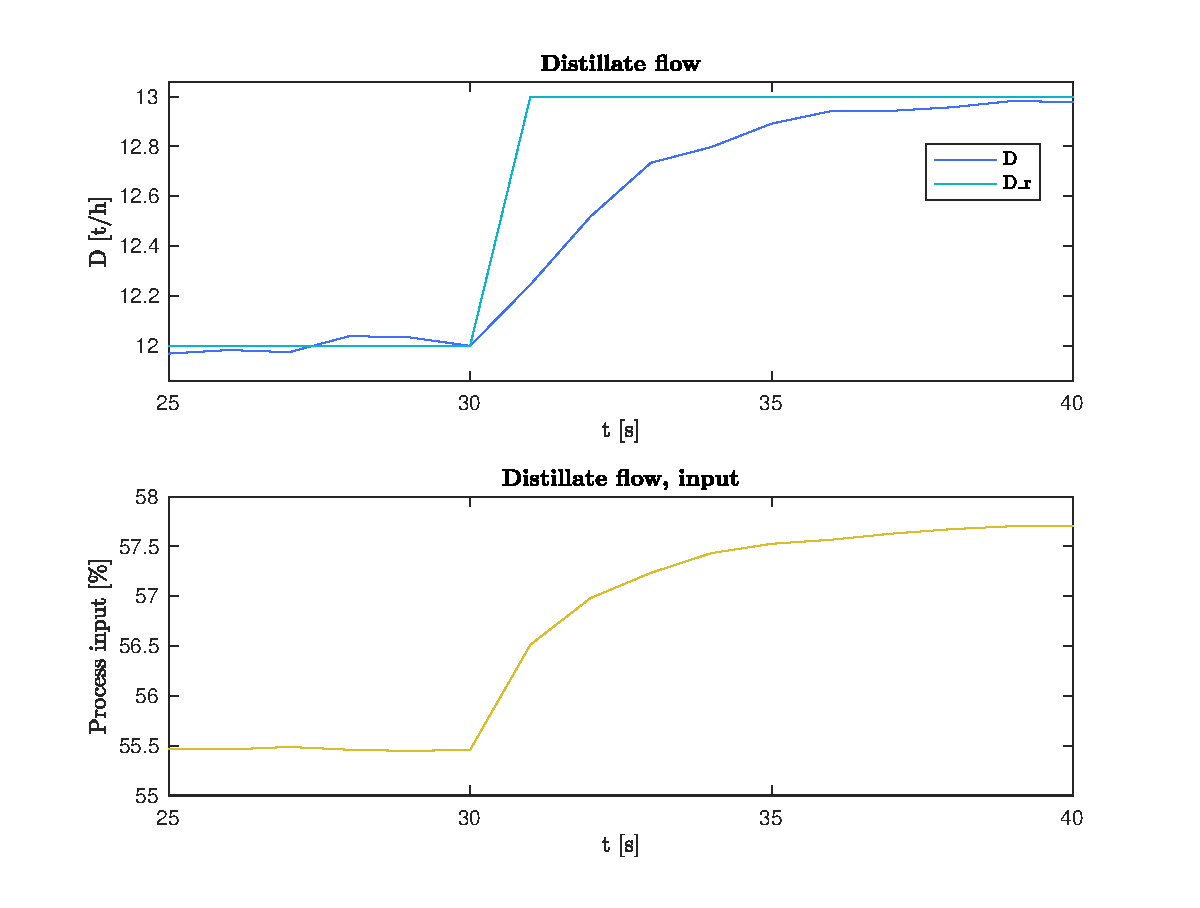
\includegraphics[width=0.8\textwidth]{../Systemanalyse/Log_Data_to_Matlab/Figurer/Stegeksperimenter/FC1005_step.eps}
\caption{Closed-loop step response of $D$}
\label{fig:cl_step_FC1005}
\end{figure}

\begin{figure}[p]
\centering
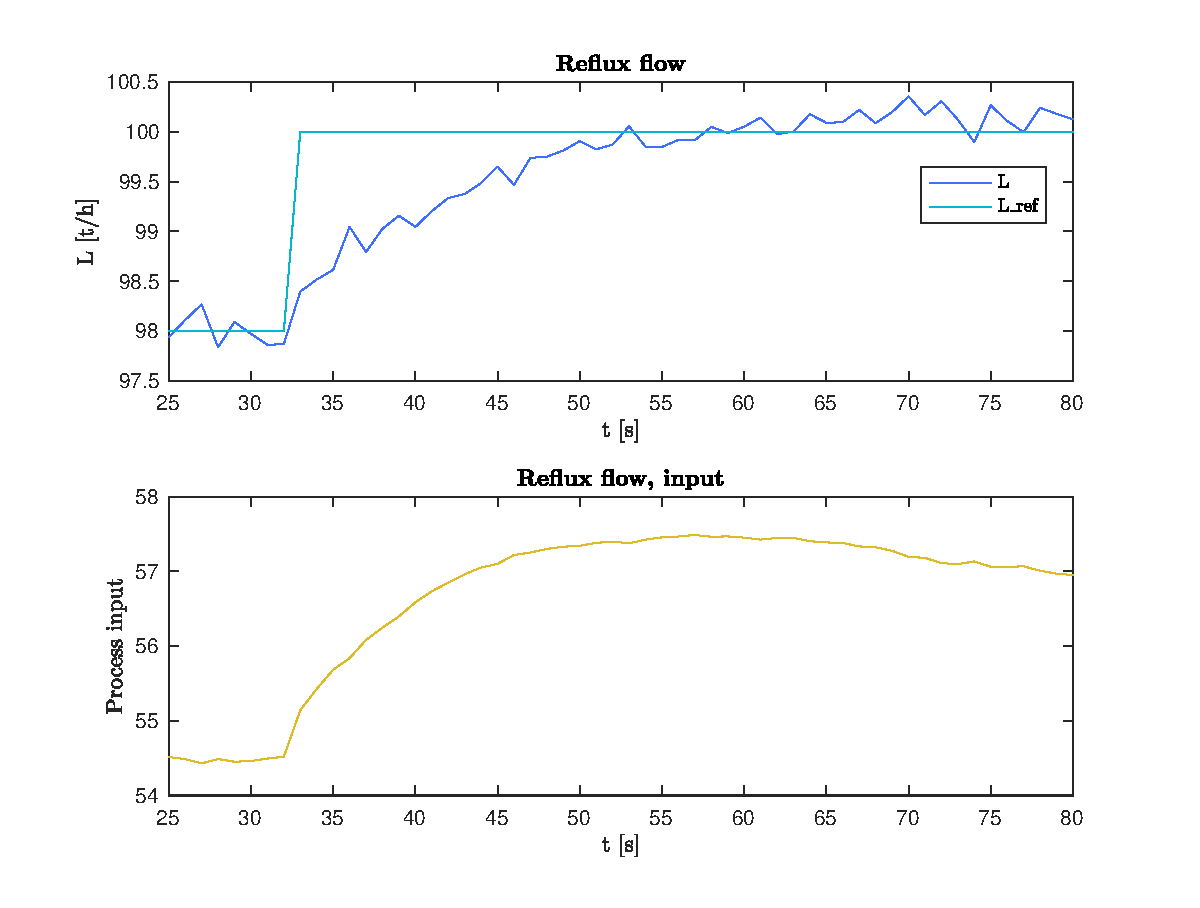
\includegraphics[width=0.8\textwidth]{../Systemanalyse/Log_Data_to_Matlab/Figurer/Stegeksperimenter/FC1015_step.eps}
\caption{Closed-loop step response of $L$}
\label{fig:cl_step_FC1015}
\end{figure}

\begin{figure}[p]
\centering
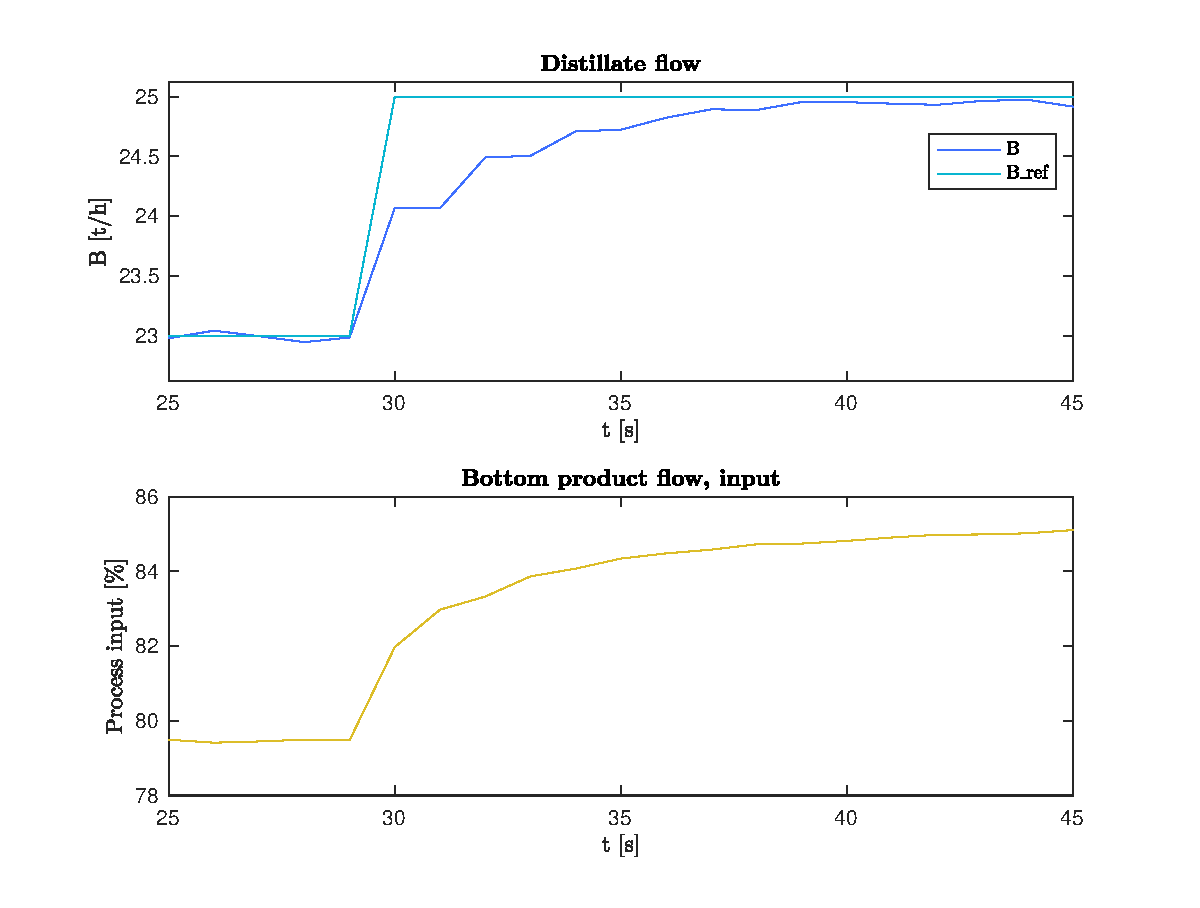
\includegraphics[width=0.8\textwidth]{../Systemanalyse/Log_Data_to_Matlab/Figurer/Stegeksperimenter/FC1019_step.eps}
\caption{Closed-loop step response of $B$}
\label{fig:cl_step_FC1019}
\end{figure}

\begin{figure}[p]
\centering
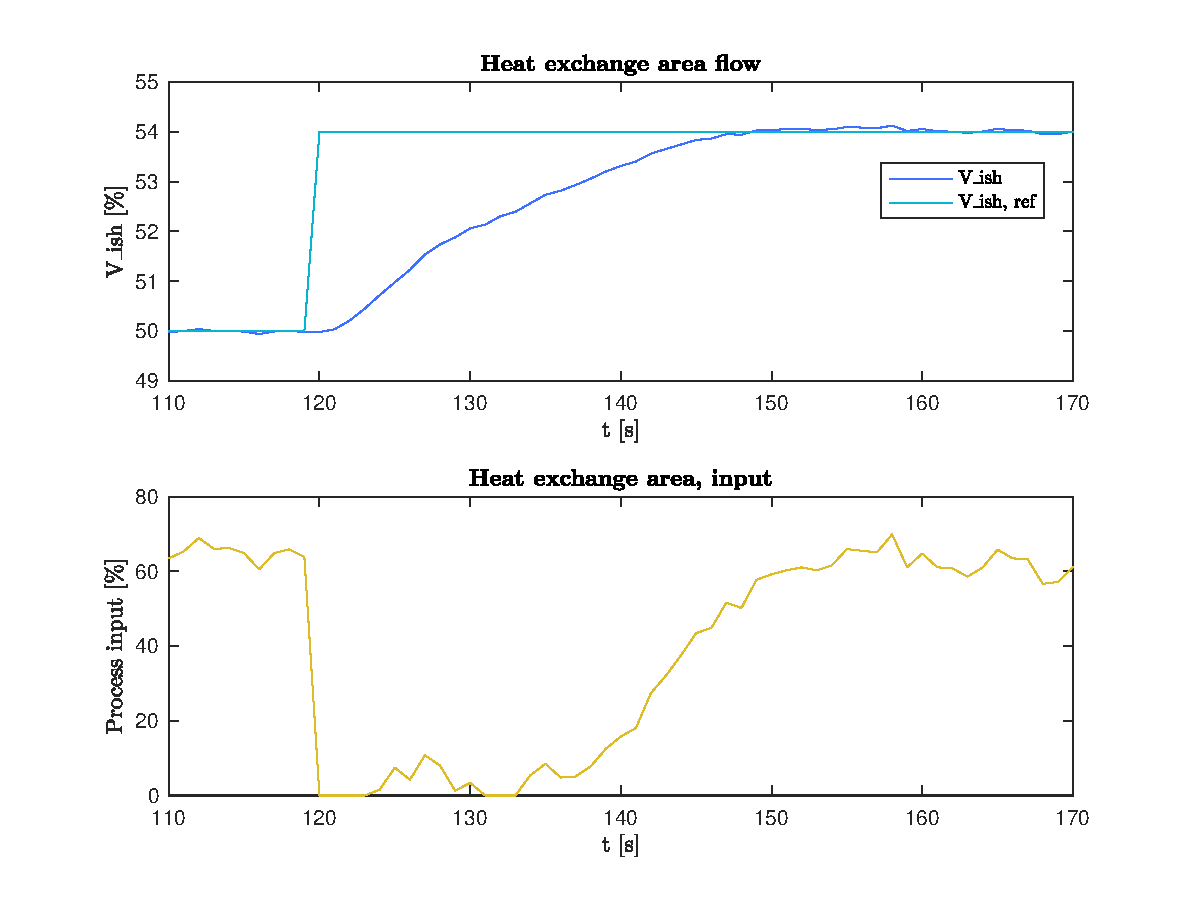
\includegraphics[width=0.8\textwidth]{../Systemanalyse/Log_Data_to_Matlab/Figurer/Stegeksperimenter/LC1028_step.eps}
\caption{Closed-loop step response of heat exchanger area, related to $V$}
\label{fig:cl_step_LC1028}
\end{figure}

\begin{figure}[p]
\centering
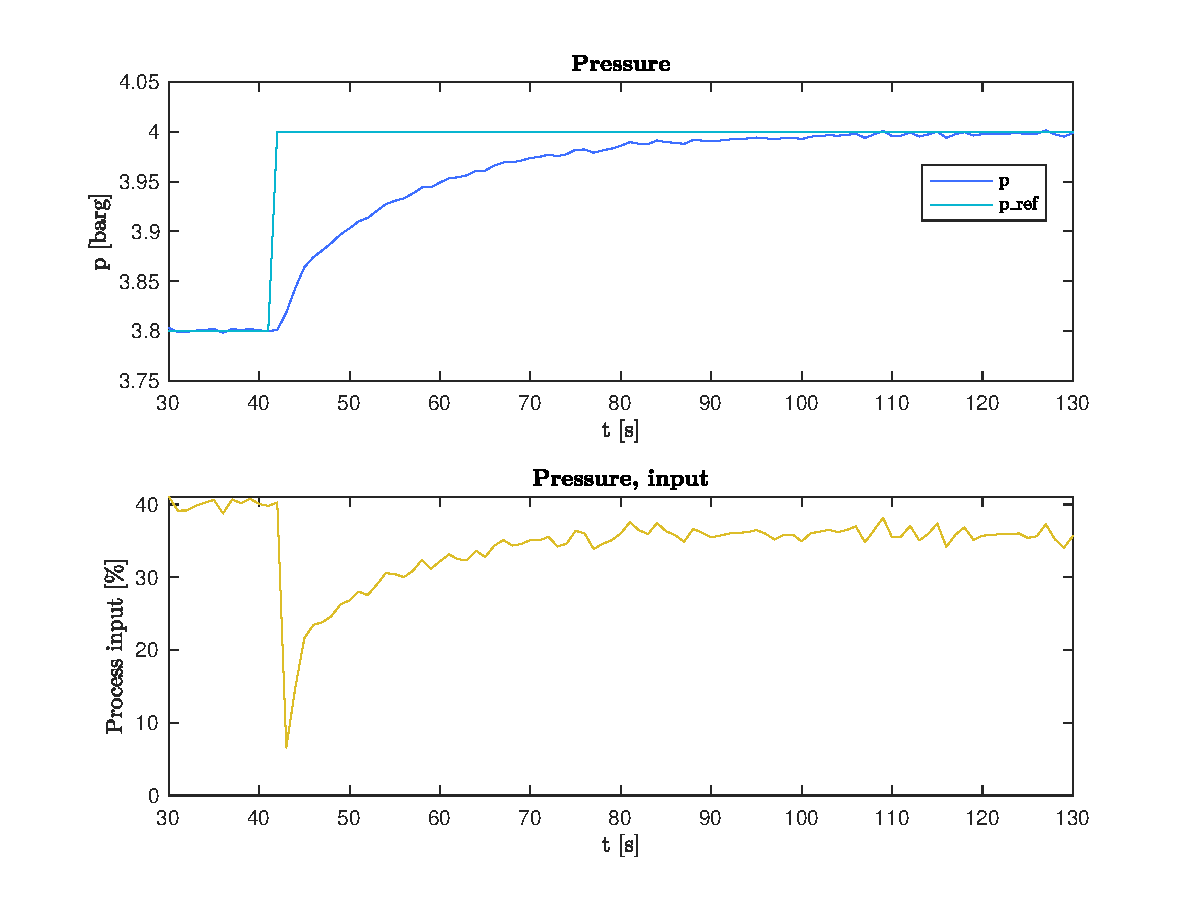
\includegraphics[width=0.8\textwidth]{../Systemanalyse/Log_Data_to_Matlab/Figurer/Stegeksperimenter/PC1024_step.eps}
\caption{Closed-loop step response of $p$}
\label{fig:cl_step_PC1024}
\end{figure}


\newpage
\section{Level controllers}
The level controllers were identified using the \texttt{d-sr} toolbox on the closed-loop responses of the level control loops in the reflux drum, and in the distillation column.

\subsection{Notation}
The system being analysed in the sectioon consists of the input $u = [D \quad B]^T$, the state $y = [M_D \quad M_B]^T$ and the reference $r = [M_{D, \textrm{ref}} \quad M_{B, \textrm{ref}}]^T$. By exciting the controlled system
\begin{equation}
y(s) = L(s)e(s) = G(s) K(s) (y(s) - r(s))
\end{equation}
with changes in $r$, the loop transfer function $L(s) = \frac{y}{e}(s)$ may be identified. Choosing $K(s)$ to be diagonal during the identification experiment makes further analysis and controller tuning easier.

\subsection{System identification and analysis}
\subsubsection{Experiment}
The level controllers in the distillation column and reflux drum were expected to be more or less independent, but MIMO identification with \texttt{d-sr} was used anyway, due to the convenience of being able to reuse code in the composition control task. Data from K-spice was imported using the script delivered together with the assignment. This data was then analyzed using the following Matlab code

\begin{verbatim}
% State vector is y = [M_D; M_B], with corresponding input u = [D; B];
Y = [LC1016(:, 1), LC1015(:, 1)];
U = [LC1016(:, 2)-LC1016(:, 1), LC1015(:, 2)-LC1015(:, 1)];
% Dimensional limit parameter
L = 3;

[A,B,C,D,CF,F,x0]=dsr(Y,U,L);
\end{verbatim}

The discrete-time system returned from \texttt{d-sr} was then transformed to the loop transfer function used in frequency analysis below by the following code

\begin{verbatim}
sample_time = min(diff(Time));
disc_system = ss(A, B, C, D, sample_time);
cont_system = d2c(disc_system);

A = cont_system.A;
B = cont_system.B;
C = cont_system.C;
D = cont_system.D;

[G_i1_num, G_i1_den] = ss2tf(A, B, C, D, 1);
[G_i2_num, G_i2_den] = ss2tf(A, B, C, D, 2);

l11 = tf(G_i1_num(1, :), G_i1_den);
l12 = tf(G_i2_num(1, :), G_i2_den);
l21 = tf(G_i1_num(2, :), G_i1_den);
l22 = tf(G_i2_num(2, :), G_i2_den);

L = [l11 l12; l21 l22];
RGA = L .* inv(L).';
\end{verbatim}

The system was excited by step changes in references for $M_D$ and $M_B$, which were controlled with P controllers, both with $K_p = 1200$. The references were changed at different periods, to better extract information about all frequencies. The states were attempted held in a reasonable interval, to avoid nonlinear effects such as saturation. The experiments are shown in figures \ref{fig:MD_experiment} and \ref{fig:MB_experiment}.

\subsubsection{Analysis}
The identified model was chosen to have order 2, which is natural for what was expected to be a diagonal system with two variables. The interactions of the resulting system is shown in figure \ref{fig:BD_RGA}, which show the RGA of the identified $G(s)$. Inspecting this plot shows that the magnitudes of the off-diagonal elements are negligible at frequencies above $10^{-3} \frac{\textrm{rad}}{\textrm{s}}$. We shall see that this is well below the bandwith frequencies of the two loops. The diagonal elements of the RGA however, have gain close to unity at the bandwith frequencies. From here, the level controller system is considered to be diagonal, and the control loops are tuned independently using SISO methods. Continuing using MIMO notation, a diagonal controller
\begin{equation}
K(s) =
\begin{bmatrix}
k_1(s) & 0\\
0 & k_2(s)
\end{bmatrix}
\end{equation}
with PI controllers $k_1(s)$ and $k_2(s)$ is designed based on the diagonal elements in the identified $G(s)$.

Figures \ref{fig:L11} and \ref{fig:L22} show the Bode plots of the transfer functions in the diagonals of the identified model. Note that these correspond to the loop transfer function $G(s) K(s)$ using a P controller with $K_p = 1200$. The controller derived here therefore has to be multiplied with this existing $K(s)$ when implemented.

Ignoring the $360^\circ$ error in phase in the plots, the gain margin of loop transfer function $l_{11}(s) = \frac{M_D}{M_{D, ref}}(s)$ may be found to be to be 6,74dB as $\omega \rightarrow \infty$. Likewise, the gain margin of $l_{22}(s) = \frac{M_B}{M_{B, ref}}(s)$ is read to be 10,7dB as $\omega \rightarrow \infty$. Using the 6dB gain margin rule of thumb (which is often used in \cite{regtek}), $K_{p, D}$ should not be increased by any significant amount, while $K_{p, B}$ might be increased by a factor of $10^{(10,7-6)/20} \approx 1,7$, yielding the controller gain $K_{p, B} = 2000$.

The phase plot of $l_{11}$ shows that the integral part of the controller should be active in the lower frequency spectrum. To avoid the phase crossing the $-180^\circ$ line, the choice of $T_i = 5000s$ is made. The phase response of $l_{22}$ is pretty similar to the one of $l_{11}$, so initially choosing the same integral time for control of $M_B$ should be reasonable.

Figures \ref{fig:S1} and \ref{fig:S2} show the magnitudes of the sensitivity functions for the two systems using these controllers. The distillation column is, not surprisingly, the hardest system of the two to control quickly. One might wish to push the bandwith of the $M_B$ loop further to the right, but inspecting the phase plot again suggests not to attempt this. This is because the phase margin would be dangerously low $K_p$ was increased or $T_i$ was decreased, and the system would become more sensitive to time delays and similar phenomena. Disturbances at frequencies above $0,005 \frac{\textrm{rad}}{\textrm{s}}$ should hopefully not be common in this system anyway.


\begin{figure}[p]
\centering
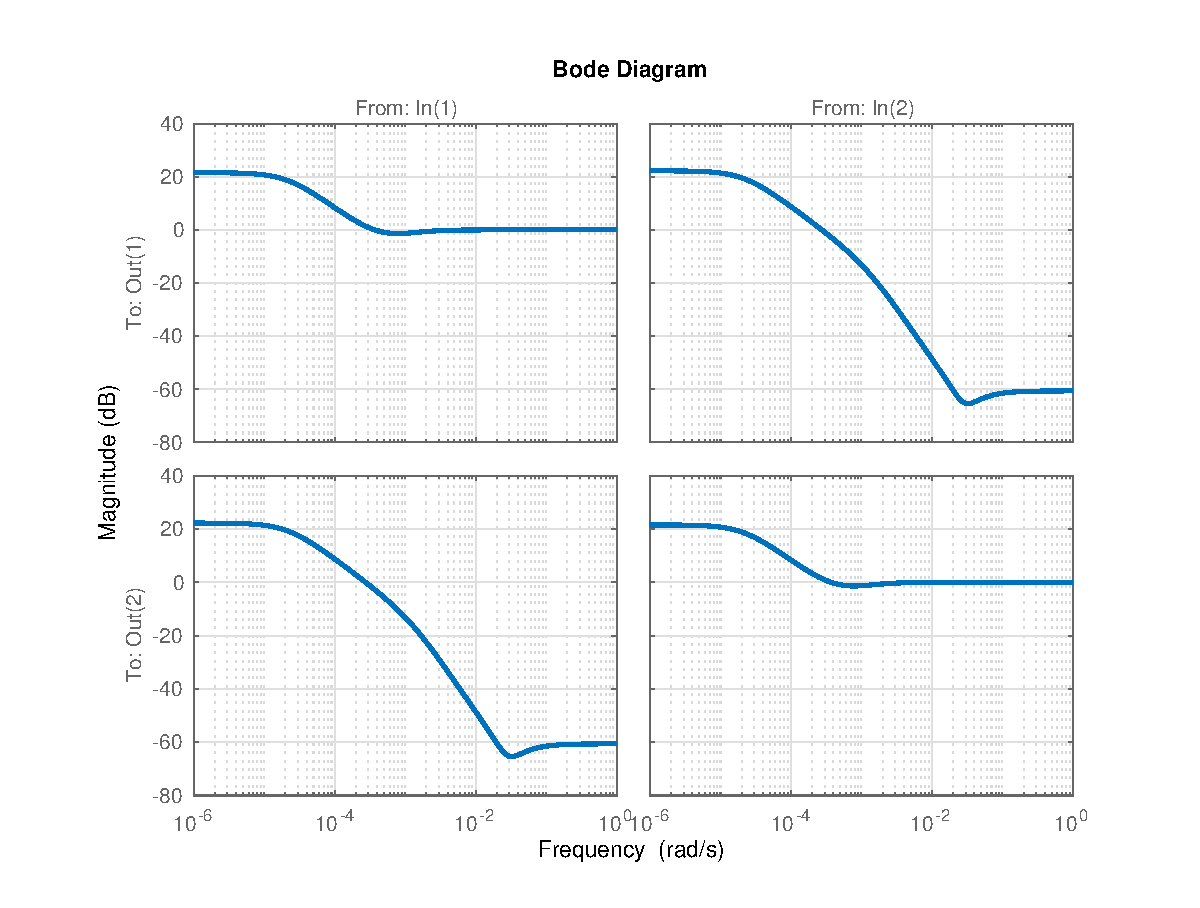
\includegraphics[width=\textwidth]{../Systemanalyse/Log_Data_to_Matlab/Figurer/Identifisering/BD_RGA.eps}
\caption{Magnitude of RGA of identified BD system}
\label{fig:BD_RGA}
\end{figure}

\begin{figure}[p]
\centering
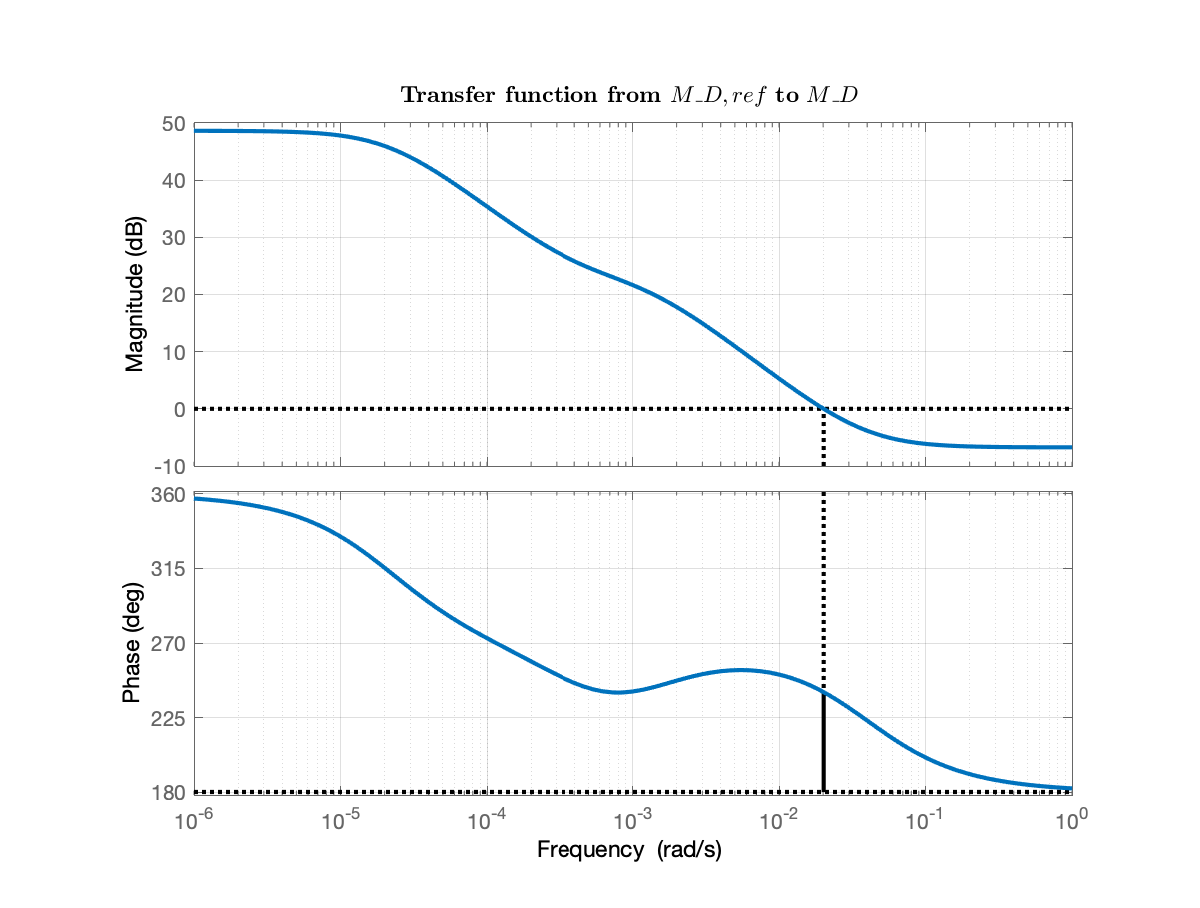
\includegraphics[width=0.8\textwidth]{../Systemanalyse/Log_Data_to_Matlab/Figurer/Identifisering/MD_bode.eps}
\caption{Magnitude and phase response of reflux drum level from reflux drum level reference}
\label{fig:L11}

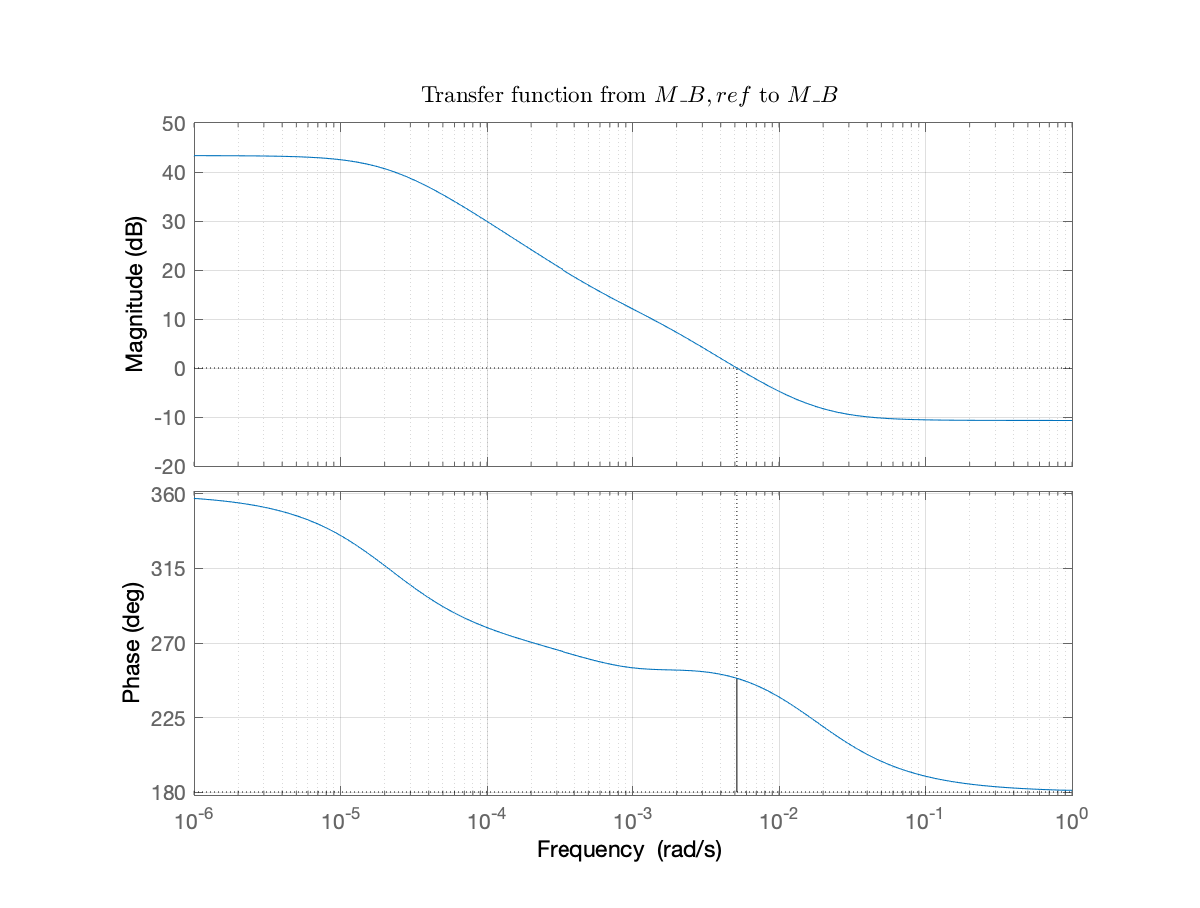
\includegraphics[width=0.8\textwidth]{../Systemanalyse/Log_Data_to_Matlab/Figurer/Identifisering/MB_bode.eps}
\caption{Magnitude and phase response of distillation column level from distillation column level reference}
\label{fig:L22}
\end{figure}

\begin{figure}[p]
\centering
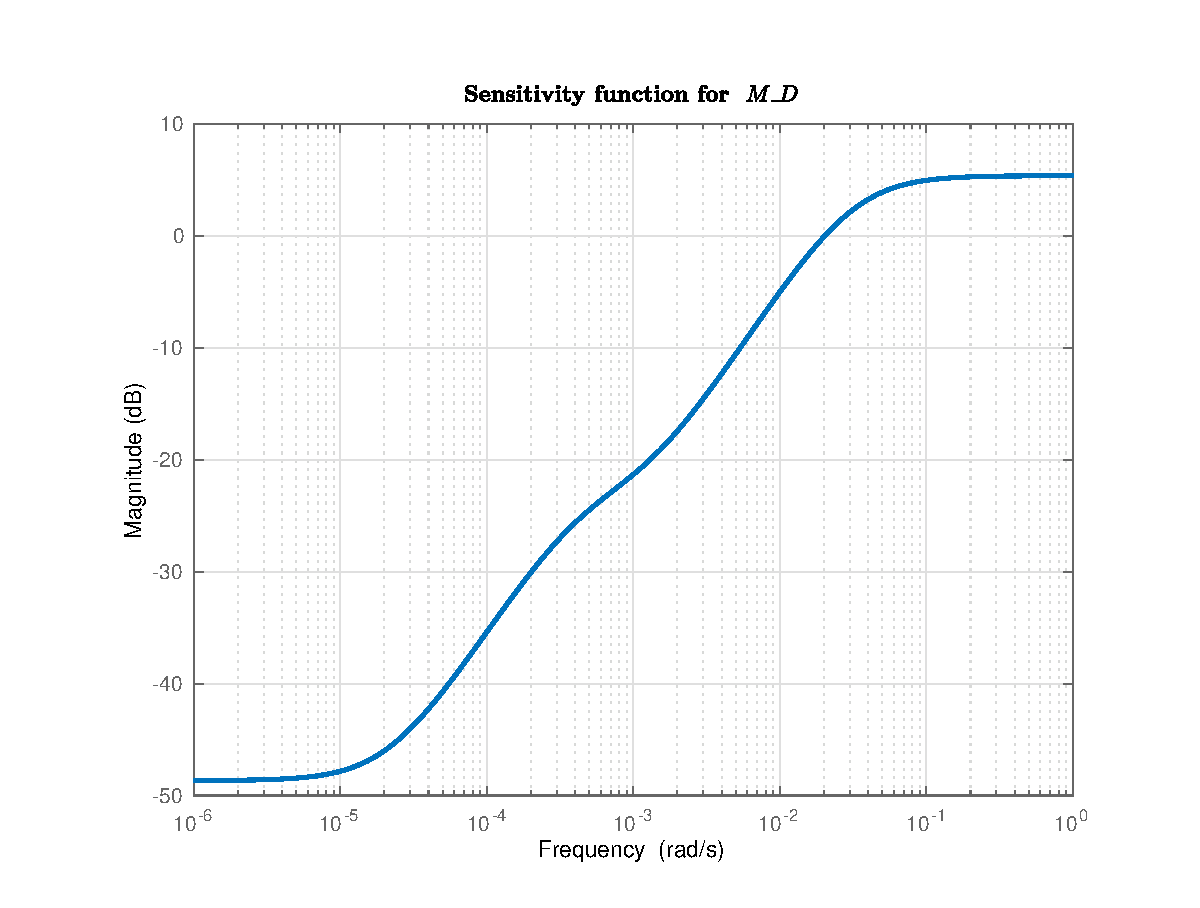
\includegraphics[width=0.8\textwidth]{../Systemanalyse/Log_Data_to_Matlab/Figurer/DB_tuning/S1.eps}
\caption{Sensitivity function for reflux drum level control}
\label{fig:S1}

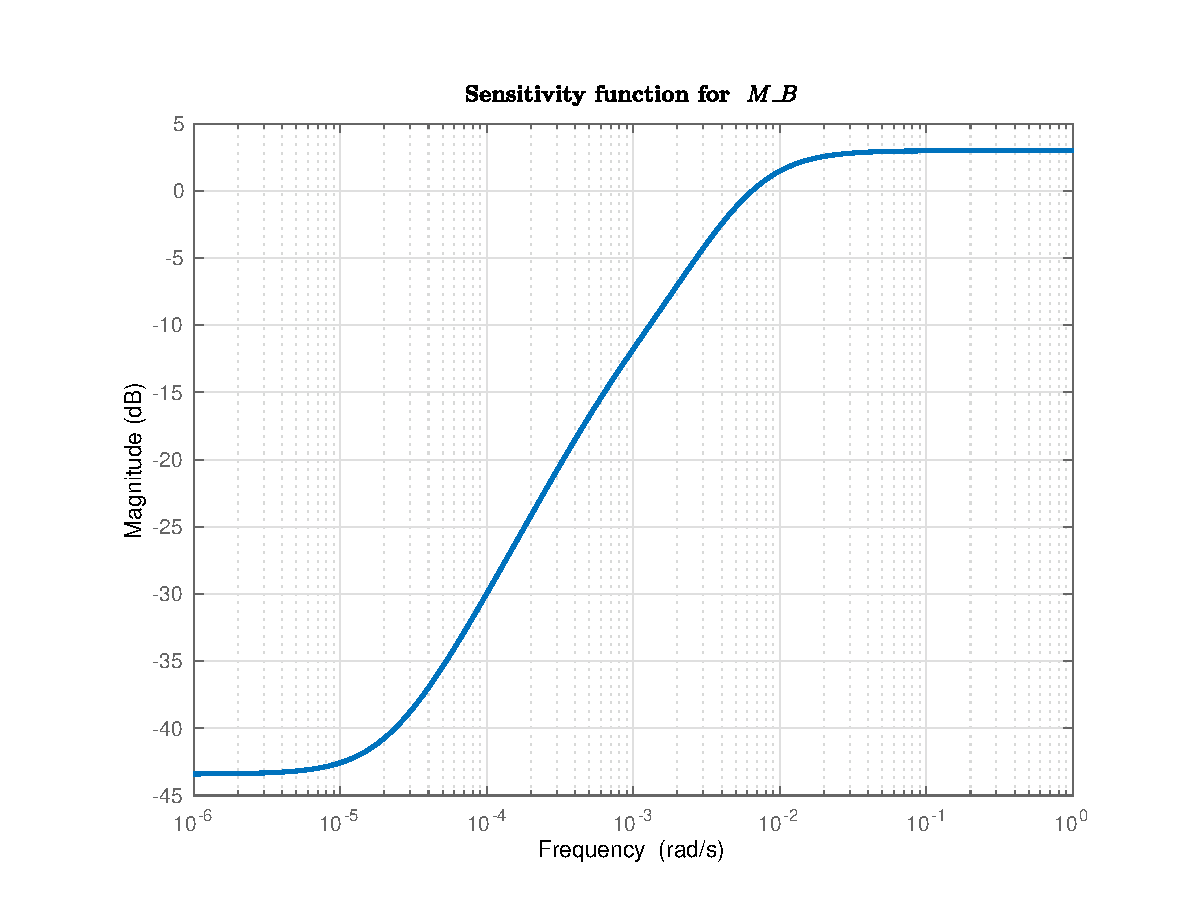
\includegraphics[width=0.8\textwidth]{../Systemanalyse/Log_Data_to_Matlab/Figurer/DB_tuning/S2.eps}
\caption{Sensitivity function for distillation column level control}
\label{fig:S2}
\end{figure}

\subsection{Controller tuning}
Simulation in K-spice showed stationary deviation in $M_D$. To counteract this, the integral time was reduced. Control of $M_B$ worked satisfactory using the PI controller derived from the frequency analysis above. The slow time constants of these systems combined with the complexity of the K-spice model, made tuning based on the K-spice model unpractical. It's natural to believe that access to more computing power would make it possible to find better controller parameters, but the controllers derived in from the analysis above didn't seem to be too terrible.

The initial parameters based on loop-shaping, and the final ones are shown in table \ref{tab:DB_parameters}. The step responses of the controlled levels are shown in figures \ref{fig:MD_step} and \ref{fig:MB_step}.

\begin{table}[h]
\centering
\begin{tabular}{c | c | c : c | c}
 & $K_{p, \textrm{initial}}$ & $T_{i, \textrm{initial}}$ & $K_{p, \textrm{final}}$ & $T_{i, \textrm{final}}$\\ \hline
 $M_D$ & 1200 & 5000s & 1200 & 1000s \\
 $M_B$ & 2000 & 5000s & 2000 & 5000s
\end{tabular}
\caption{Parameters for level controllers}
\label{tab:DB_parameters}
\end{table}

\begin{figure}[p]
\centering
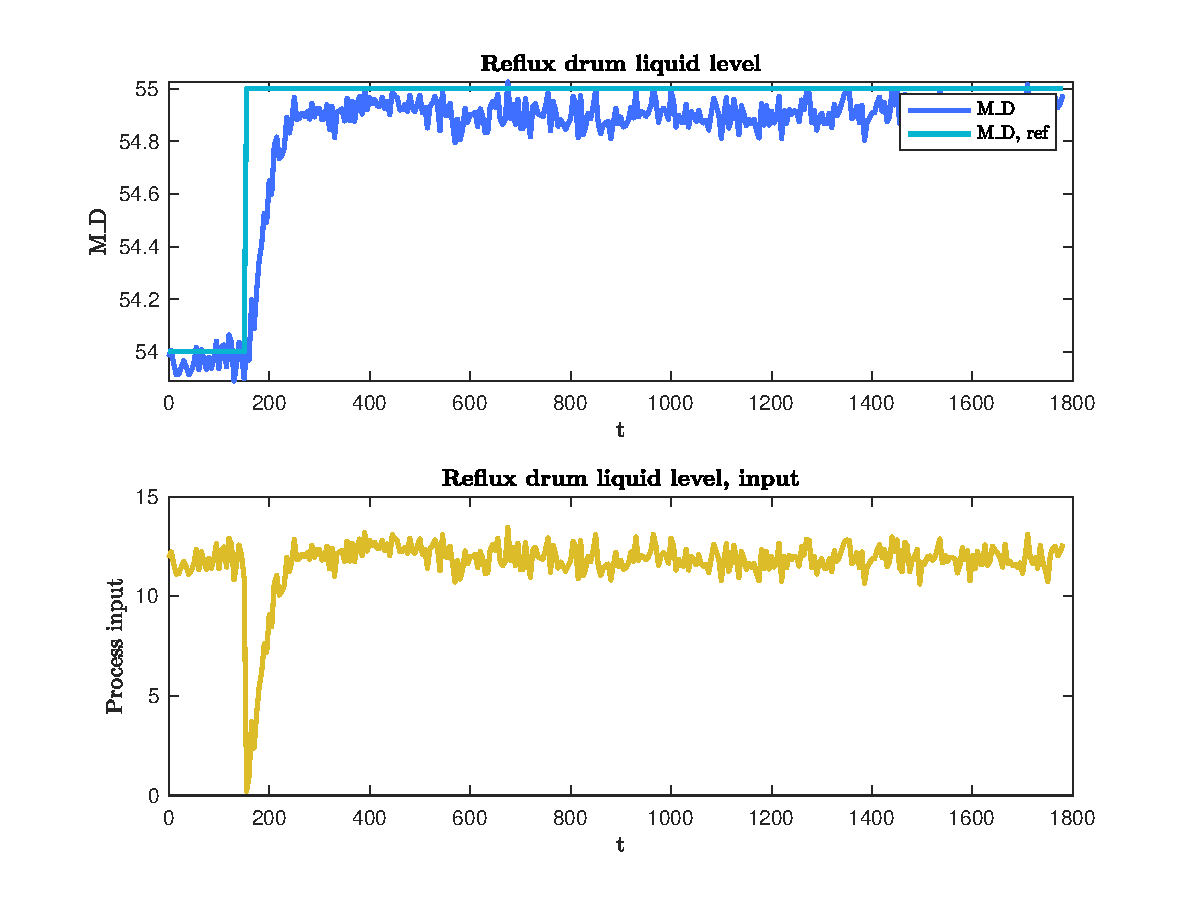
\includegraphics[width=0.8\textwidth]{../Systemanalyse/Log_Data_to_Matlab/Figurer/Identifisering/M_D_with_M_D_step.eps}
\caption{Step response of controlled $M_D$}
\label{fig:MD_step}
\end{figure}

\begin{figure}
\centering
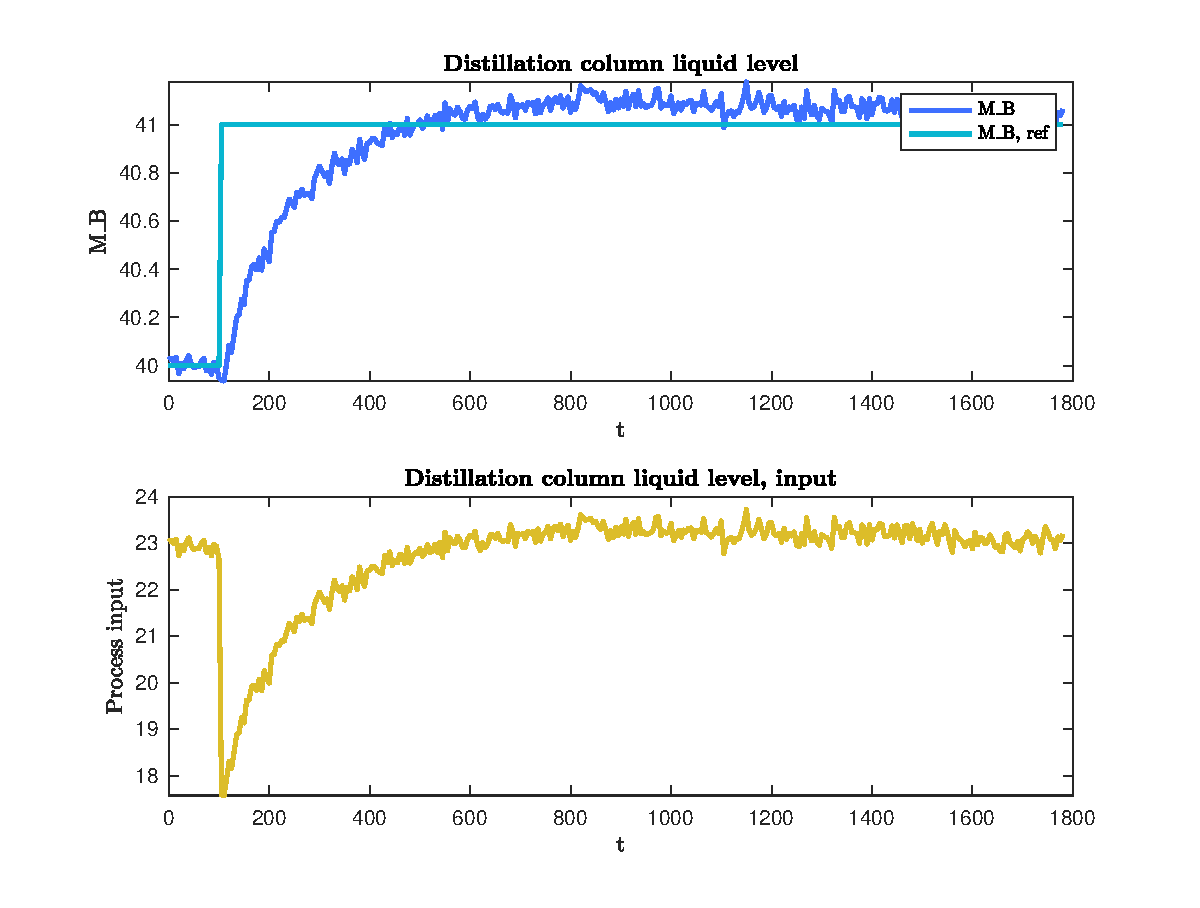
\includegraphics[width=0.8\textwidth]{../Systemanalyse/Log_Data_to_Matlab/Figurer/Identifisering/M_B_with_M_B_step.eps}
\caption{Step response of controlled $M_B$}
\label{fig:MB_step}
\end{figure}

\newpage
\section{Composition controllers}
Let $y = [T_D \quad T_B]^T$, $r = [T_{D, \textrm{ref}} \quad T_{B, \textrm{ref}}]^T$ and $u = [L \quad V]^T$. By changing the setpoints for the manipulated variables $L$ and $V$, the system transfer function
\begin{equation}
G(s) = \frac{y}{u}(s)
\end{equation}
may be identified directly.
\subsection{System identification and analysis}
\subsubsection{Experiment}
Identification of the LV system was done in a similar manner as in the previous section, using step changes in input (but open-loop this time). Again, \texttt{d-sr} was used for identification. The periods of the step changes were chosen more systematically than in the level experiment, with periods of 5 minutes, 15 minutes and $\approx2$ minutes being used for different periods of time. This was done to get an accurate representation of the system at all frequencies. The inputs $L$ and $V$ were changed alternatingly (i.e. $90^\circ$ out of phase), to avoid ambiguity in which input caused what effects. Figure \ref{fig:LV_experiment} shows the inputs ($L$ and $V$) and resulting outputs ($T_D$ and $T_B$) in the experiment. Simlarly to the previous section, the code used for identification was as follows

\begin{verbatim}
% State vector is y = [T_D; T_B], with corresponding input u = [L; V];
Y = [TC1015(:, 1), TC1088(:, 1)];
U = [FC1015(:, 1), LC1028(:, 1)];

% Scaling is done to keep all signals in the range [0, 1]
Y = (Y - 25*ones(size(Y))) * [1/25 0; 0 1/25];
U = U * [1/120 0; 0 1/100];

% Dimensional limit parameter
G = 3;

[A,B,C,D,CF,F,x0]=dsr(Y,U,G);
\end{verbatim}
The code used to get the system transfer function $G(s)$ was identical to the code used in the previous system.

\subsubsection{Analysis}
Figure \ref{fig:LV_RGA} shows the RGA of the identified system $G(s) = \frac{y}{u}(s)$. The chosen pairing is clearly the most reasonable. The interactions doesn't seem to be any problem, but the RGA doesn't tell the whole story. There is reason to believe that temperature in the bottom affects temperature in the top, and the right tool for this analysis is the \textit{Performance Relative Gain Array} (PRGA).

Let $\tilde{G} = \textrm{diag}\{g_{ii}\}$, i.e. the matrix consisting of only the diagonal elements of the system matrix. This matrix is a useful tool for analysing interactions, and is used in the definition of the PRGA

\begin{equation}
\Gamma = \tilde{G} G^{-1}
\end{equation}
This matrix is used as a measure of interaction. It is scaling dependent, so before any further analysis is done, this has to be taken into account. Given a subsystem

\begin{equation}
e = y - r = G(s) u + G_d(s) d - r
\end{equation}
the signals should be scaled such that the maximum expected disturbance and maximum acceptable error both are of magnitude one. Table \ref{tab:LV_scaling} shows the range used in K-spice for the states in the temperature control loops, and maximum accepted error. To be clear, the following analysis holds for both control loops, with $y$ being temperature, $r$ reference temperature, and $u$ process input. The maximum error allowed is chosen based on the lowest margin proposed in the assignment text. Disturbance rejection is not considered because it is assumed that no disturbance will be greater than the disturbance coming from interaction between the loops. This effect is handled if we manage to keep $| e | < 1$.

The PRGA using this scaling is shown in figure \ref{fig:LV_PRGA}. It is now clear that one can't simply choose a bandwith of $0,01 \frac{\textrm{rad}}{\textrm{s}}$ and call it a day, since the interaction from $V$ to $T_D$ has its peak at this frequency.

What should be done, then? Since we're dealing with a MIMO system, only using the diagonal parts of $G$ for designing controllers won't suffice. Our main objectives is to follow the reference. In \cite{skogestad}, some rules for designing independent controllers for MIMO systems are proposed. One of these considers reference tracking, and is used here.

For effecient reference tracking in a SISO system, an error magnitude $| e(j \omega) |$ less than one is achieved when

\begin{equation}
| S(j \omega) R | < 1
\end{equation}
for reference changes of magnitude $R$, for all frequencies $\omega$ up to the maximum frequency $\omega_r$ where good reference tracking is required. More explicitly, this requirement can be stated as

\begin{equation}
| 1 + L(j \omega) | > R
\label{eq:SISO_performance_requirement}
\end{equation}
The situation for a MIMO system is a bit more complicated when we have interactions like shown above. This is where the PRGA is useful. It is shown in \cite{skogestad} that the MIMO analogue of equation \ref{eq:SISO_performance_requirement} can be stated, using the PRGA, as

\begin{equation}
| 1 + L_i | > | \gamma_{ij} | \cdot |R_j|
\end{equation}
Here, $L_i = g_{ii}k_i$ is the loop transfer function in loop $i$, and $R_j$ is the magnitude of the reference change in loop $j$.

Assuming $R_1 = R_2 = 1$ (which should hold for our rescaled system), the requirements are as plotted in figures \ref{fig:L1_performance1} and \ref{fig:L2_performance1}, using $L_i = G_i$ (P controllers with unit gain). Inspecting these, it becomes clear that the state most desperately in need of better control is $T_D$. This is not surprising, since the PRGA showed the effect of $T_B$ on $T_D$ being large, while the effect the other way was more or less negligible. Hence, suppressing the effects $T_B$ has on $T_D$ is our most important task, while the control of $T_B$ should be relatively problem free if the controller parameters aren't chosen completely ridiculously. To shape $| 1 + L_1 |$, the integral time was first changed. $T_i = 100$s turned out to give a low maximum distance between $| 1 + L_1 |$ and $| \gamma_{1i} |$. $K_p$ was then chosen to be as small as possible while still satisfying the criterion, yielding $K_p = 12$. This actually satisfies the criterion at all frequencies, as shown in \ref{fig:L1_performance2}.

The restriction of the $T_B$ loop being located in a higher part of the frequency spectrum gave rise to the choice of $T_i = 1000s$ for this PI controller. Though the PRGA didn't suggest interaction from $T_D$ to $T_B$ would be a problem, the loop was designed to respect the inequality $| 1 + L_2 | > | \gamma_{22} |$ for all $\omega < 10^{-2}$ (meaning interaction from $T_D$ should be suppressed). As shown in figure \ref{fig:L2_performance2} is satisfied when $K_p = 25$. A summary of the resulting controller is shown in table \ref{tab:LV_parameters}

\begin{table}[h]
\centering
\begin{tabular}{c | c | c }
 & $K_p$ & $T_i$  \\ \hline
 $T_D$ & 12 & 100s \\
 $T_B$ & 25 & 1000s
\end{tabular}
\caption{Parameters for temperature controllers}
\label{tab:LV_parameters}
\end{table}

\begin{table}[p]
\centering
\begin{tabular}{c | c | c | c}
Variable & Min & Max & Maximum magnitude \\ \hline
$T_D$ & $25^\circ$C & $50^\circ$C & $25^\circ$C \\
$T_B$ & $25^\circ$C & $50^\circ$C & $25^\circ$C \\
$T_{D, \textrm{ref}}$ & $25^\circ$C & $50^\circ$C & $25^\circ$C \\
$T_{B, \textrm{ref}}$ & $25^\circ$C & $50^\circ$C & $25^\circ$C \\
$L$ & $0 \frac{\textrm{t}}{\textrm{h}}$ & $120 \frac{\textrm{t}}{\textrm{h}}$ & $120 \frac{\textrm{t}}{\textrm{h}}$ \\
$V$ & $0\%$ & $100\%$ & $100\%$ \\
$e$ & - & - & $0,55^\circ$C
\end{tabular}
\caption{Scaling used in LV system analysis}
\label{tab:LV_scaling}
\end{table}

\begin{figure}[p]
\centering
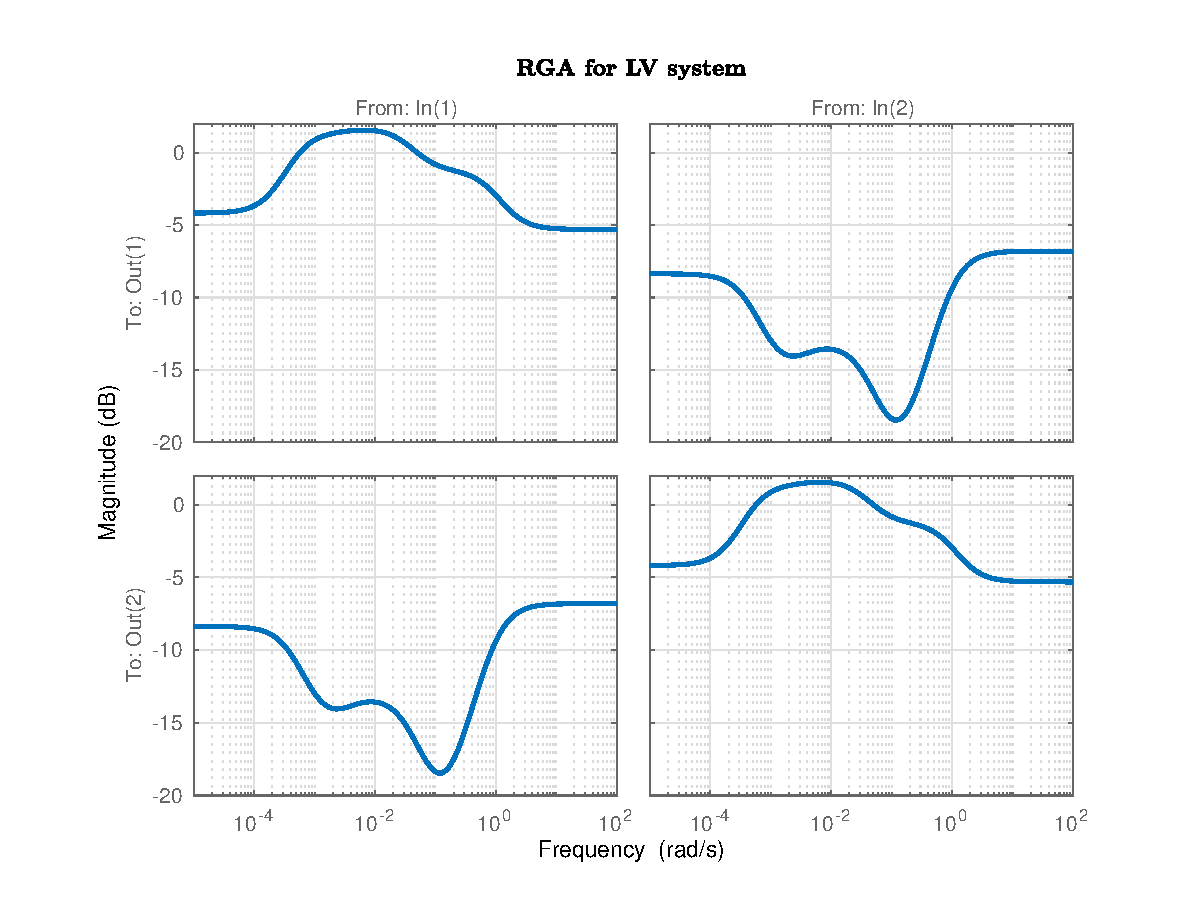
\includegraphics[width=0.8\textwidth]{../Systemanalyse/Log_Data_to_Matlab/Figurer/LV_identifisering/LV_RGA.eps}
\caption{RGA for LV system}
\label{fig:LV_RGA}

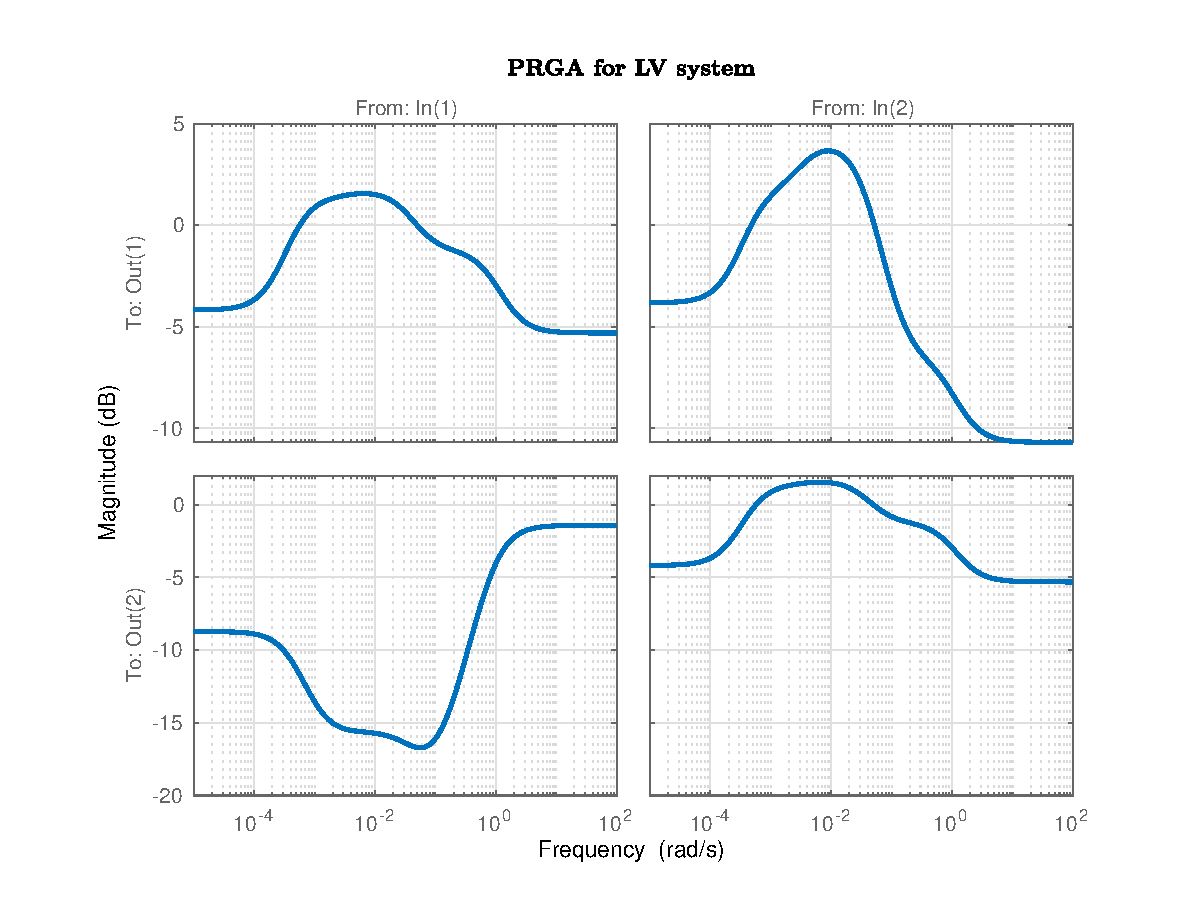
\includegraphics[width=0.8\textwidth]{../Systemanalyse/Log_Data_to_Matlab/Figurer/LV_identifisering/LV_PRGA.eps}
\caption{PRGA for LV system}
\label{fig:LV_PRGA}
\end{figure}

\begin{figure}[p]
\centering
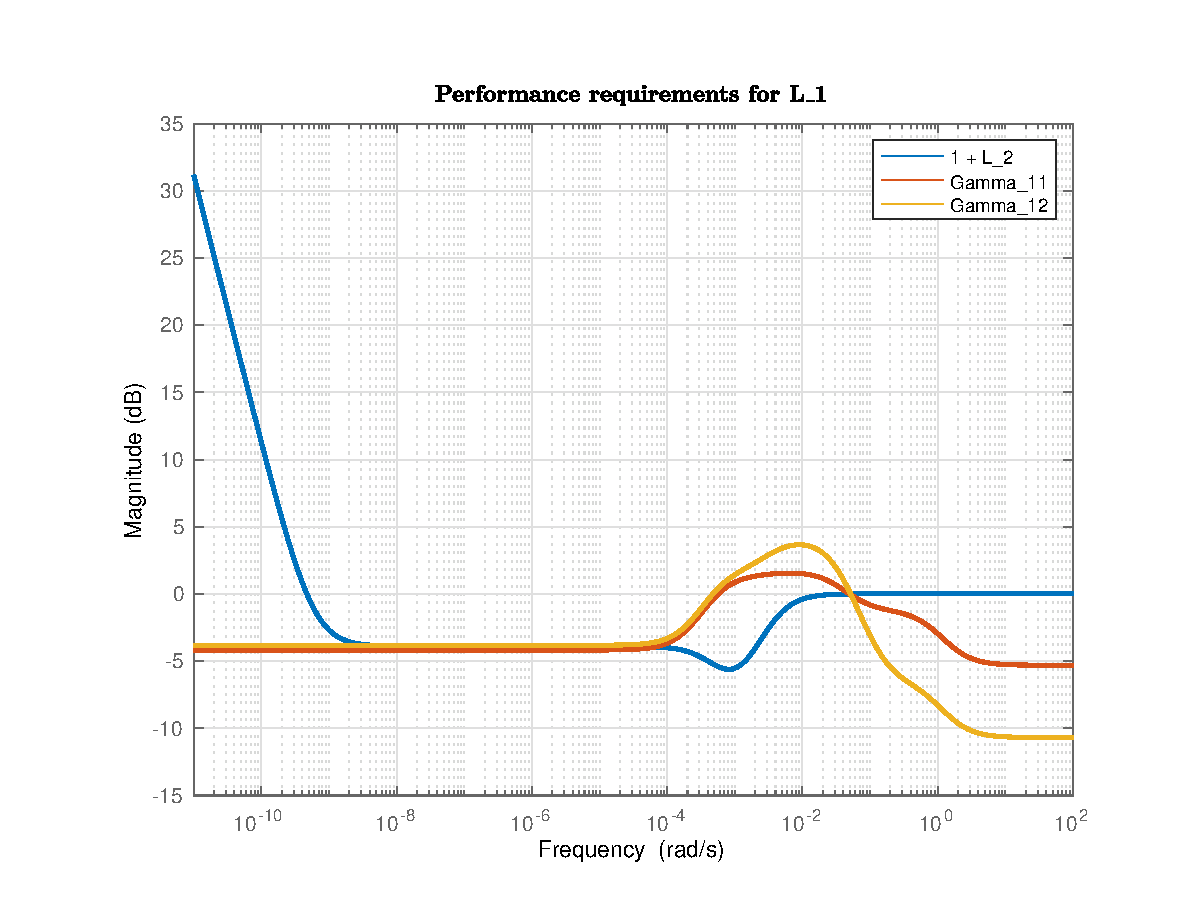
\includegraphics[width=0.8\textwidth]{../Systemanalyse/Log_Data_to_Matlab/Figurer/LV_identifisering/L1_krav_P-reg.eps}
\caption{Performance requirements for $T_D$ loop, with unit gain P controller}
\label{fig:L1_performance1}

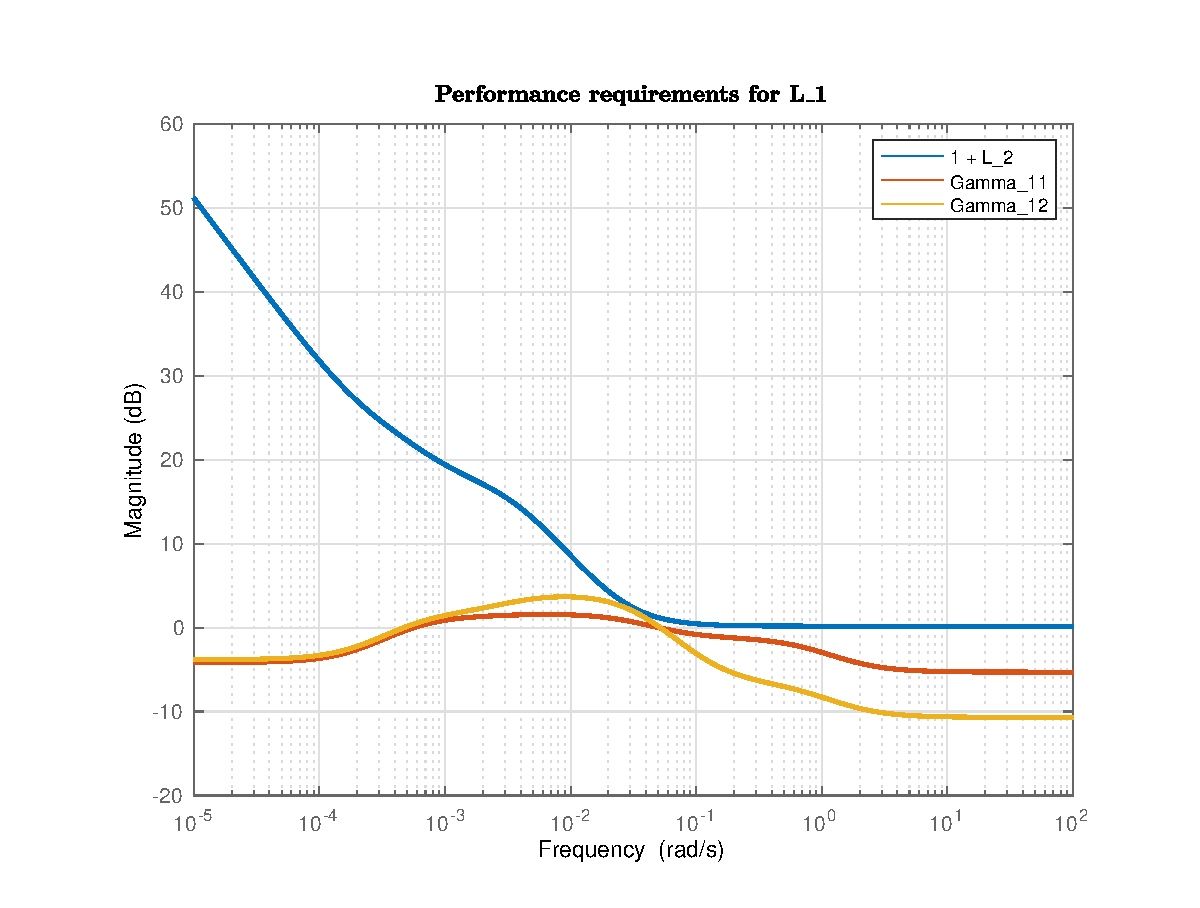
\includegraphics[width=0.8\textwidth]{../Systemanalyse/Log_Data_to_Matlab/Figurer/LV_identifisering/L1_krav_PI-reg.eps}
\caption{Performance requirements for $T_D$ loop, with implemented PI controller}
\label{fig:L1_performance2}
\end{figure}

\begin{figure}[p]
\centering
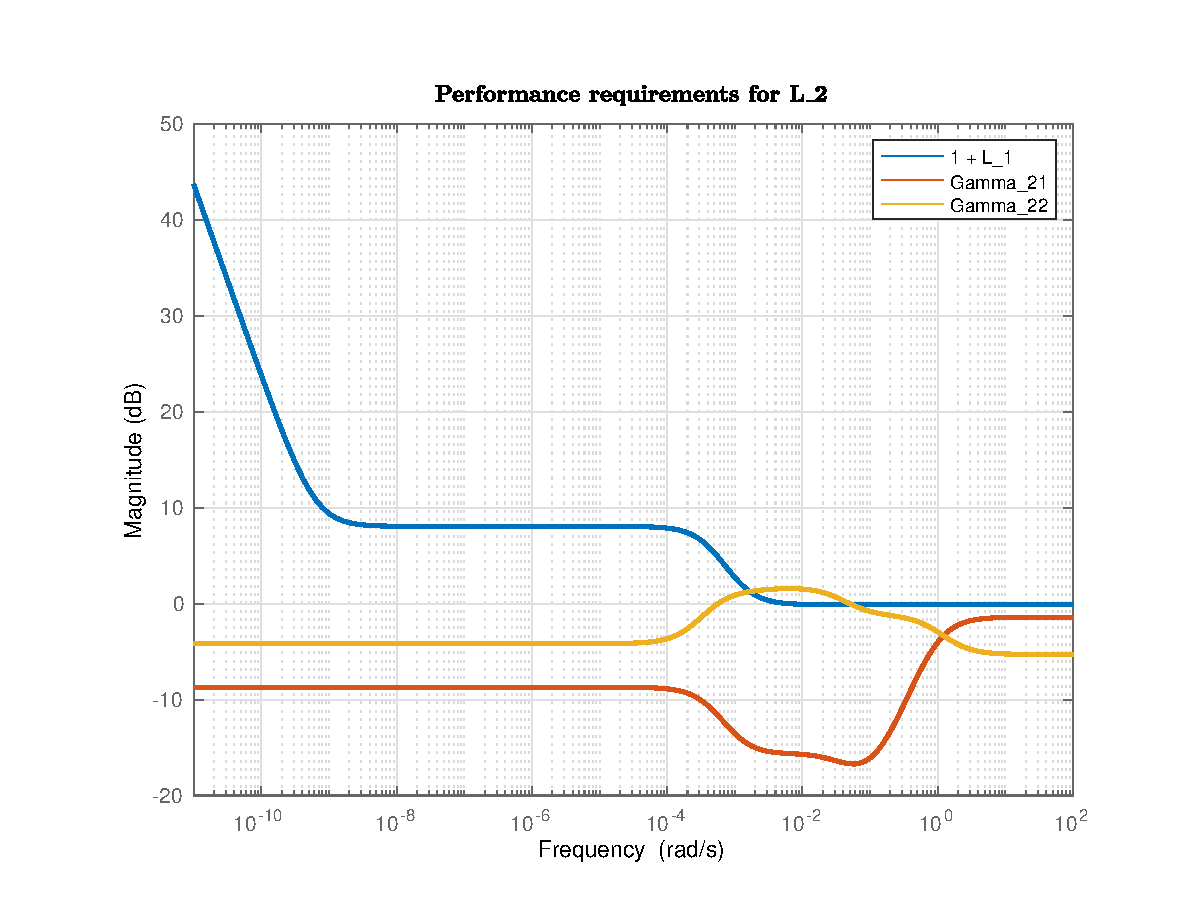
\includegraphics[width=0.8\textwidth]{../Systemanalyse/Log_Data_to_Matlab/Figurer/LV_identifisering/L2_krav_P-reg.eps}
\caption{Performance requirements for $T_B$ loop, with unit gain P controller}
\label{fig:L2_performance1}

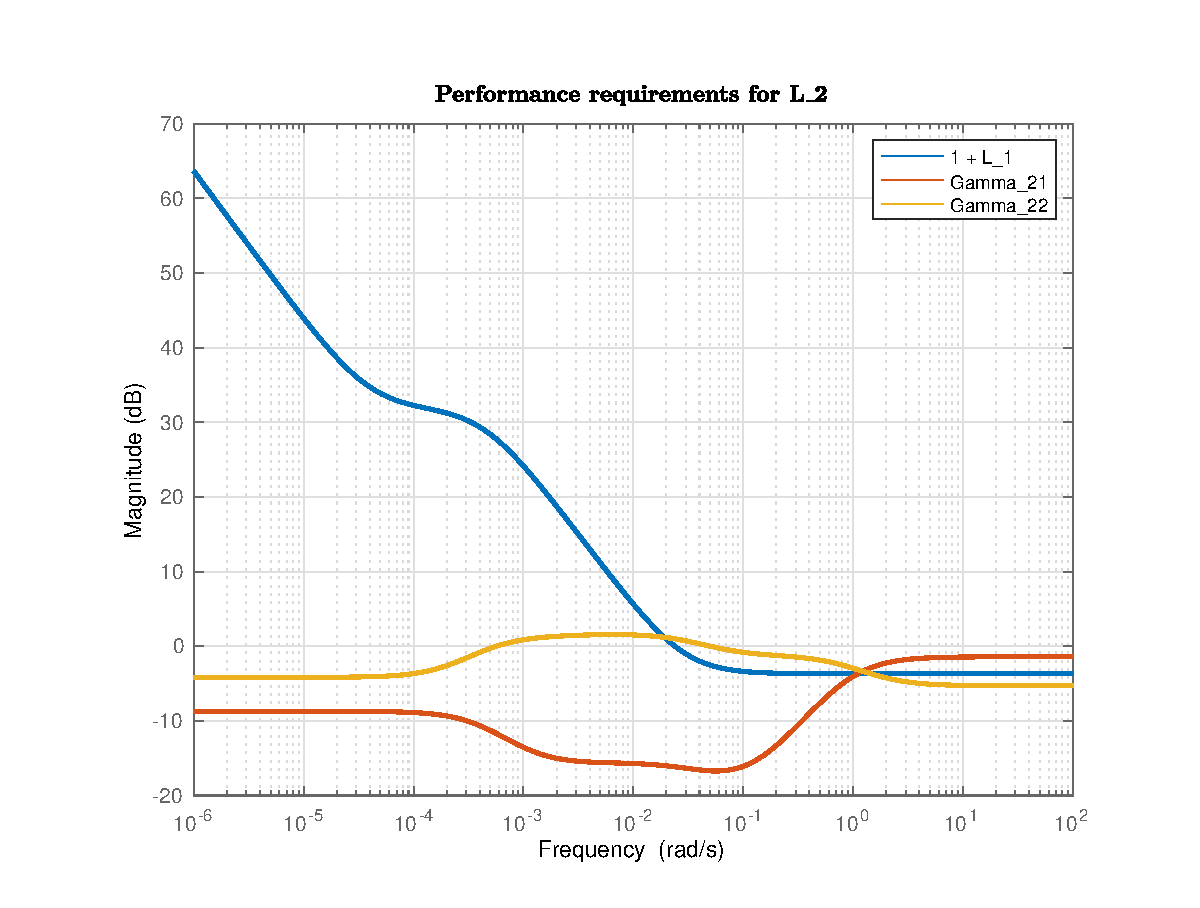
\includegraphics[width=0.8\textwidth]{../Systemanalyse/Log_Data_to_Matlab/Figurer/LV_identifisering/L2_krav_PI-reg.eps}
\caption{Performance requirements for $T_B$ loop, with implemented PI controller}
\label{fig:L2_performance2}
\end{figure}

\newpage
\section{Results}

\subsection{PI controller tuning}
Table \ref{tab:final_controller_parameters} shows the final PI controller parameters for all the control loops tuned in this project, also including the scaled gain $G$ used in the K-spice implementation.

\begin{table}[p]
\centering
\begin{tabular}{c | c | c | c }
& $K_p$ & $G$ & $T_i$ \\ \hline
$D$ (FC1005) & 0,0035 & 0,42& 0,4s\\
$L$ (FC1015) & 0,0018 & 0,22 & 1,0s \\
$B$ (FC1019) & 0,0025 & 0,3 & 1,0s \\
$V$ (LC1028) & 200 & 200 & 10s \\
$p$ (PC1024) & 5 & 30 & 20s \\
$M_D$ (LC1016) & 1200 & 10 & 1000s \\
$M_B$ (LC1015) & 2000 & 16,7 & 5000s \\
$T_D$ (TC1015) & 12 & 2,5 & 100s \\
$T_B$ (TC1088) & 25 & 6,3 & 1000s
\end{tabular}
\caption{Final controller parameters}
\label{tab:final_controller_parameters}
\end{table}


\subsection{Plots}
Figures \ref{fig:TD_TD_cl}, \ref{fig:TB_TD_cl}, \ref{fig:TD_TB_cl} and \ref{fig:TB_TB_cl} show the results of relatively large step changes in temperature reference. The system is in both cases initially operating at the least strict setpoint required to keep the product streams sufficiently pure, and one of the temperatures is then suddenly changed to the setpoint given in the rightmost column of \ref{tab:requirements}.

The plots show that there's clearly interactions in play here. However, the attempt at separating the responses in frequency seems to work. When$T_{B , \textrm{ref}}$ is increased, $T_D$ also increases. However, the $T_D$ controller quickly steers the state back to the reference, and keeps it there. This has the effect of disturbing the $T_B$ loop again, but this is the last of the interactions here. After this minor set-back, $T_B$ climbs steadily to its reference, and stays there.

A more dramatic effect is seen when $T_D$ is changed. The $T_B$ controller doesn't have the bandwith necessary suppress disturbances as quick as the step response of $T_D$. Instead, we have to rely on the interaction from $T_D$ to $T_B$ being low. The interaction is stronger stronger than what the PRGA suggested, and the disturbance causes a pretty long-lasting oscillation. Luckily, the magnitude of the oscillation is lower than the magnitude of the change in $T_{D , \textrm{ref}}$, and $T_B$ is always high enough to keep product quality satisfactory.

Though the results seem ok, there are some possible problems. The greatest one is probably the long-lasting effects of interaction from $T_D$ to $T_B$. Though the controllers could be tuned less aggressively to avoid rapid responses, this would also decrease disturbance suppression. An easier solution is to simply change the reference slower. Figures \ref{fig:TD_TD_cl_stepwise}, \ref{fig:TB_TD_cl_stepwise}, \ref{fig:TD_TB_cl_stepwise}, \ref{fig:TB_TB_cl_stepwise} show the same experiments as was just discussed, but with smaller, stepwise changes to the reference. The effects the change in $T_{B , \textrm{ref}}$ has on $T_D$ is reduced from $0,45^\circ$C to about $0,10^\circ$C. Decreasing $T_{D , \textrm{ref}}$ stepwise causes $T_B$ to oscillate with a magnitude of $0,10^\circ$C rather than $0,30^\circ$C.

This type of slow setpoint change might for instance be implemented in practice by lowpass filtering the setpoint step changes. With this implemented, the relatively aggressive controllers derived here might be kept unchanged without risking instability. This has the advantage of keeping the relatively fast settling times seen here, of around 1,5 hours for both loops.

\begin{figure}[p]
\centering
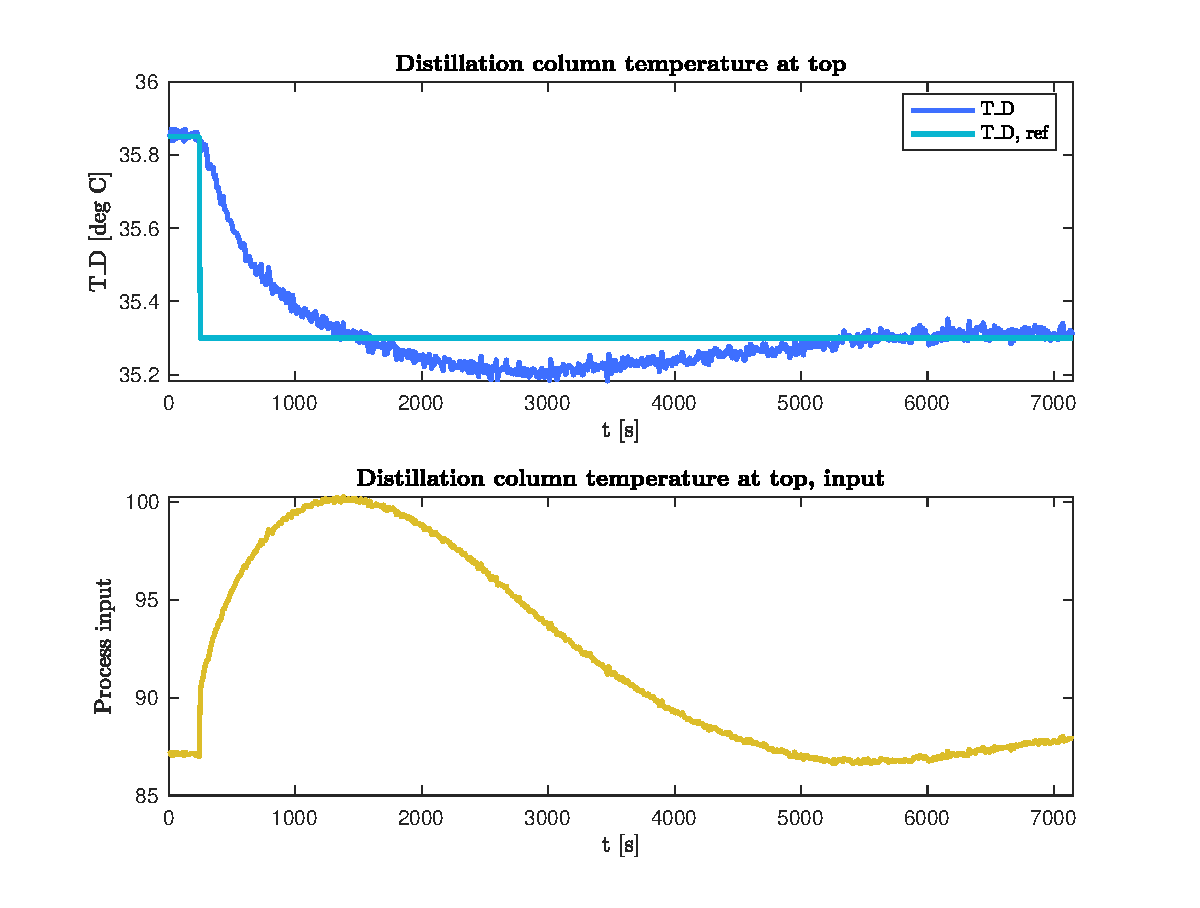
\includegraphics[width=0.8\textwidth]{../Systemanalyse/Log_Data_to_Matlab/Figurer/LV_tuning/T_D_closed_loop_with_T_D_step.eps}
\caption{Response of controlled $T_D$ to step change in $T_{D, \textrm{ref}}$}
\label{fig:TD_TD_cl}

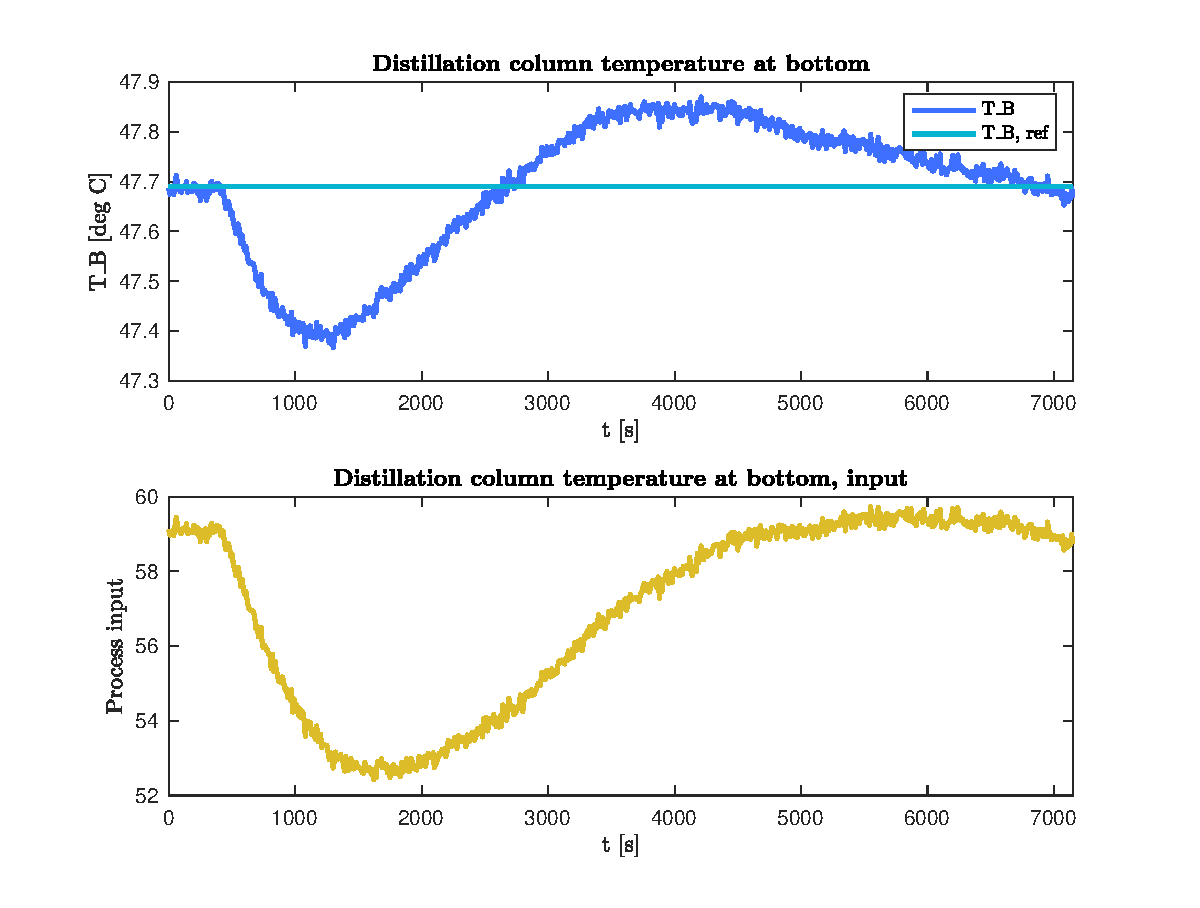
\includegraphics[width=0.8\textwidth]{../Systemanalyse/Log_Data_to_Matlab/Figurer/LV_tuning/T_B_closed_loop_with_T_D_step.eps}
\caption{Response of controlled $T_B$ to step change in $T_{D, \textrm{ref}}$}
\label{fig:TB_TD_cl}
\end{figure}

\begin{figure}[p]
\centering
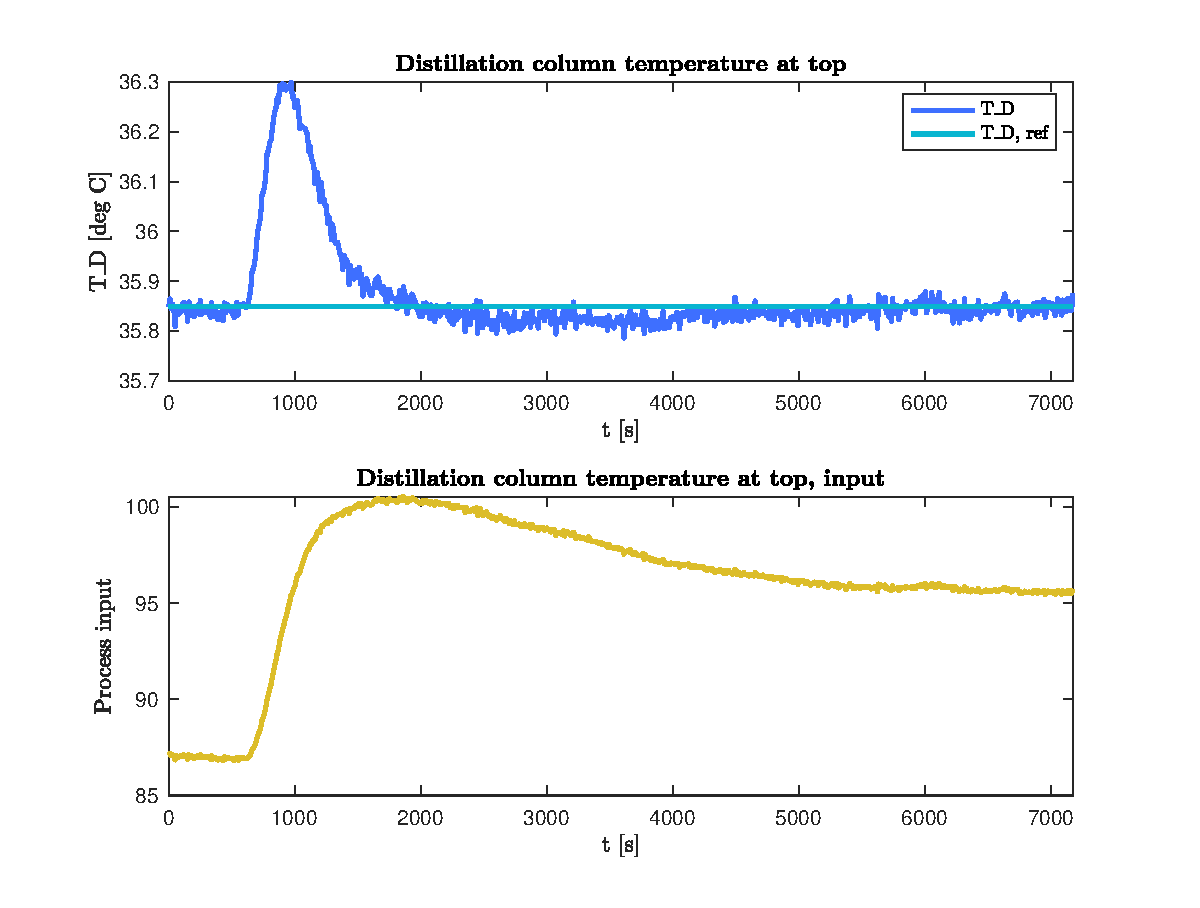
\includegraphics[width=0.8\textwidth]{../Systemanalyse/Log_Data_to_Matlab/Figurer/LV_tuning/T_D_closed_loop_with_T_B_step.eps}
\caption{Response of controlled $T_D$ to step change in $T_{B, \textrm{ref}}$}
\label{fig:TD_TB_cl}

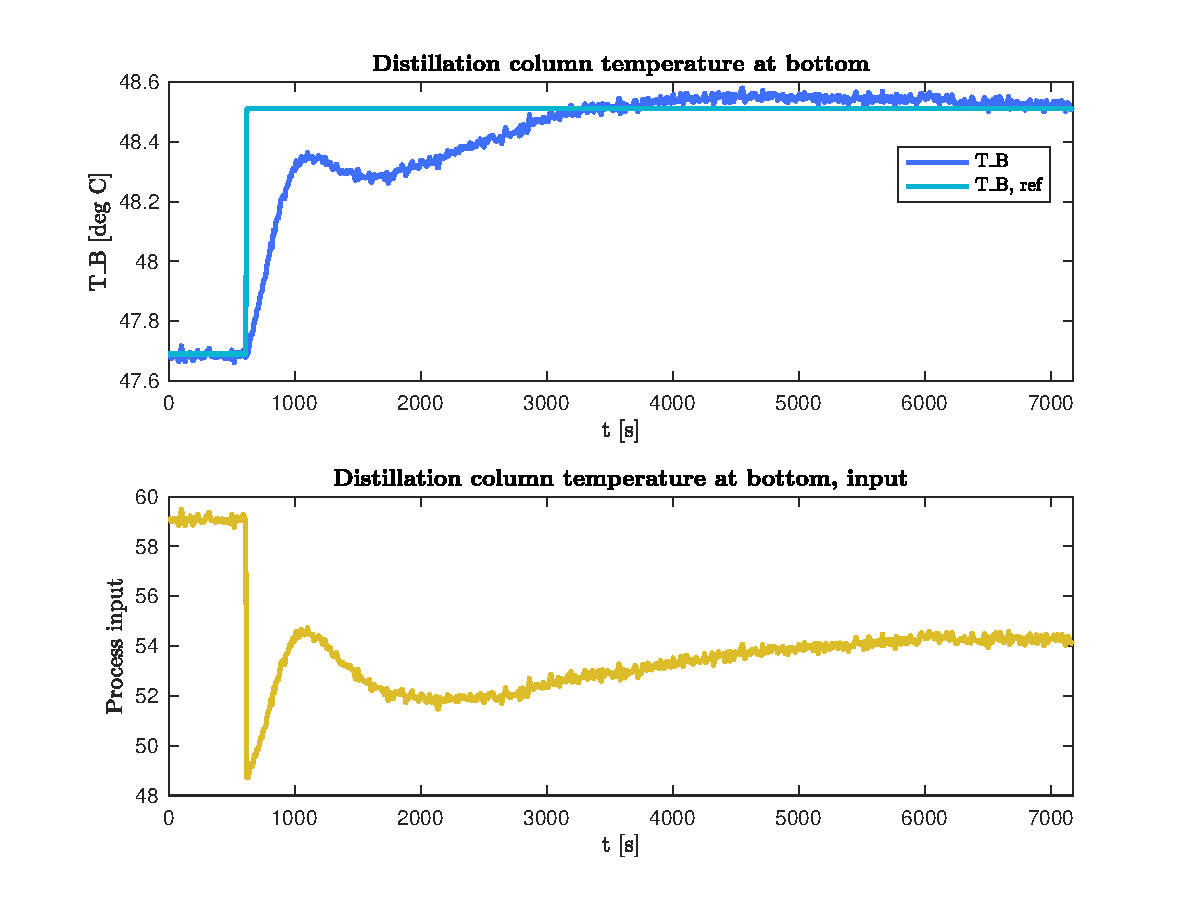
\includegraphics[width=0.8\textwidth]{../Systemanalyse/Log_Data_to_Matlab/Figurer/LV_tuning/T_B_closed_loop_with_T_B_step.eps}
\caption{Response of controlled $T_B$ to step change in $T_{B, \textrm{ref}}$}
\label{fig:TB_TB_cl}
\end{figure}


\begin{figure}[p]
\centering
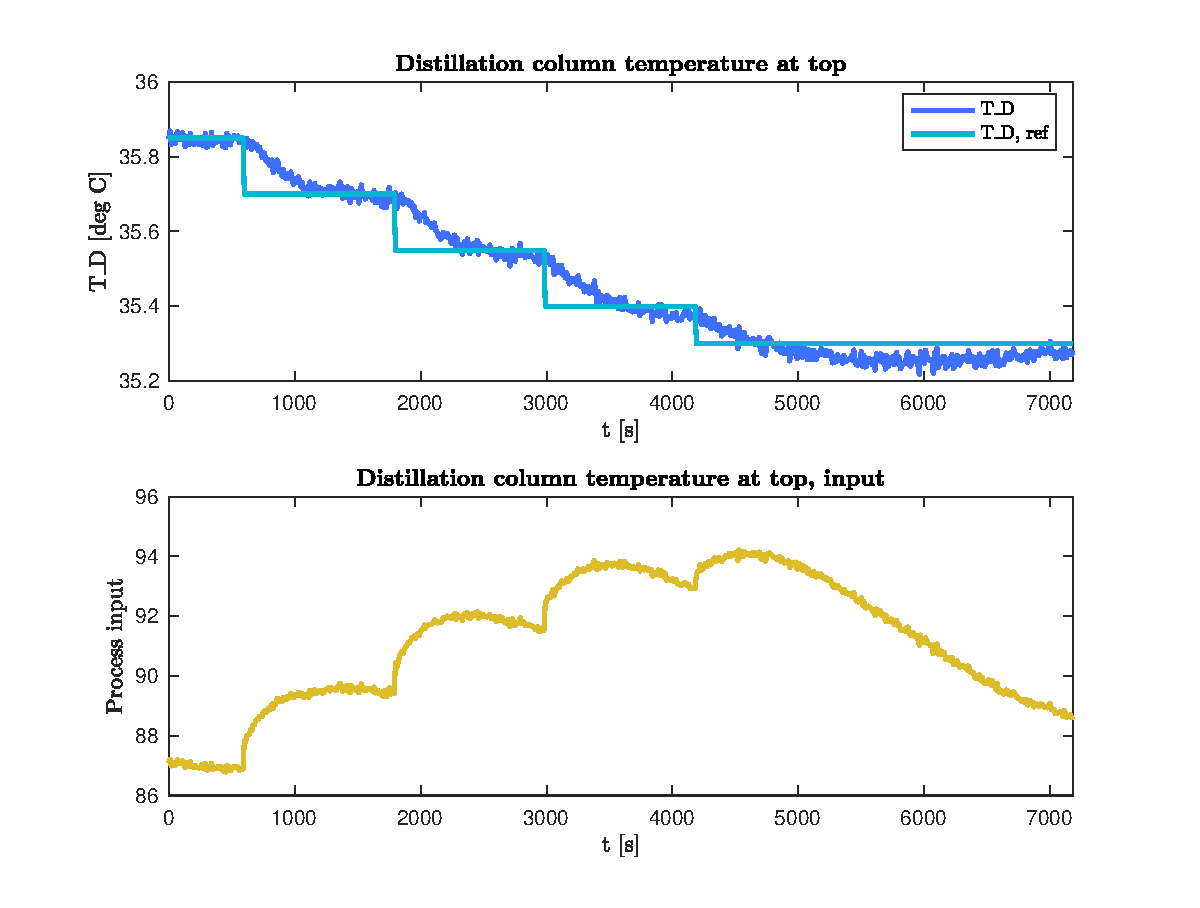
\includegraphics[width=0.8\textwidth]{../Systemanalyse/Log_Data_to_Matlab/Figurer/LV_tuning/T_D_closed_loop_with_stepwise_T_D_step.eps}
\caption{Response of controlled $T_D$ to stepwise step changes in $T_{D, \textrm{ref}}$}
\label{fig:TD_TD_cl_stepwise}

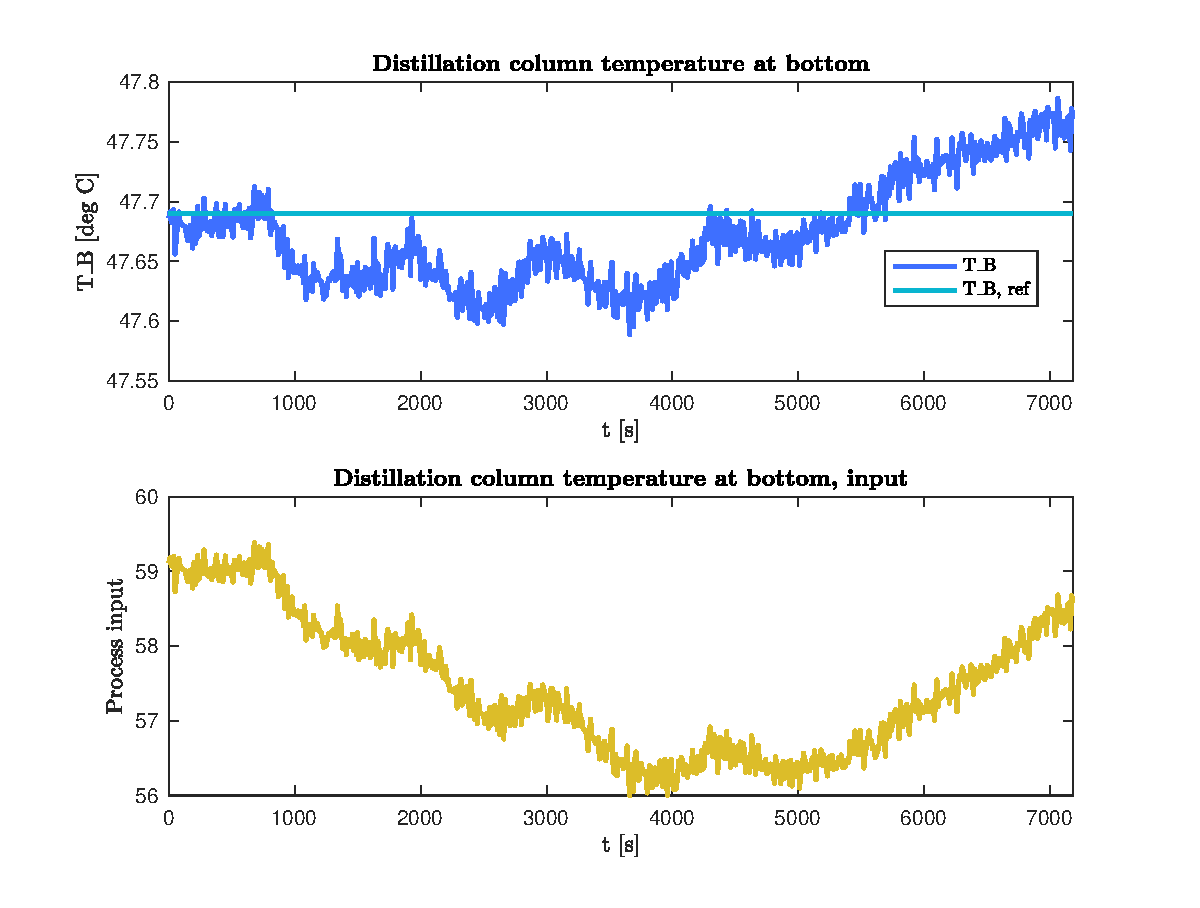
\includegraphics[width=0.8\textwidth]{../Systemanalyse/Log_Data_to_Matlab/Figurer/LV_tuning/T_B_closed_loop_with_stepwise_T_D_step.eps}
\caption{Response of controlled $T_B$ to stepwise step changes in $T_{D, \textrm{ref}}$}
\label{fig:TB_TD_cl_stepwise}
\end{figure}

\begin{figure}[p]
\centering
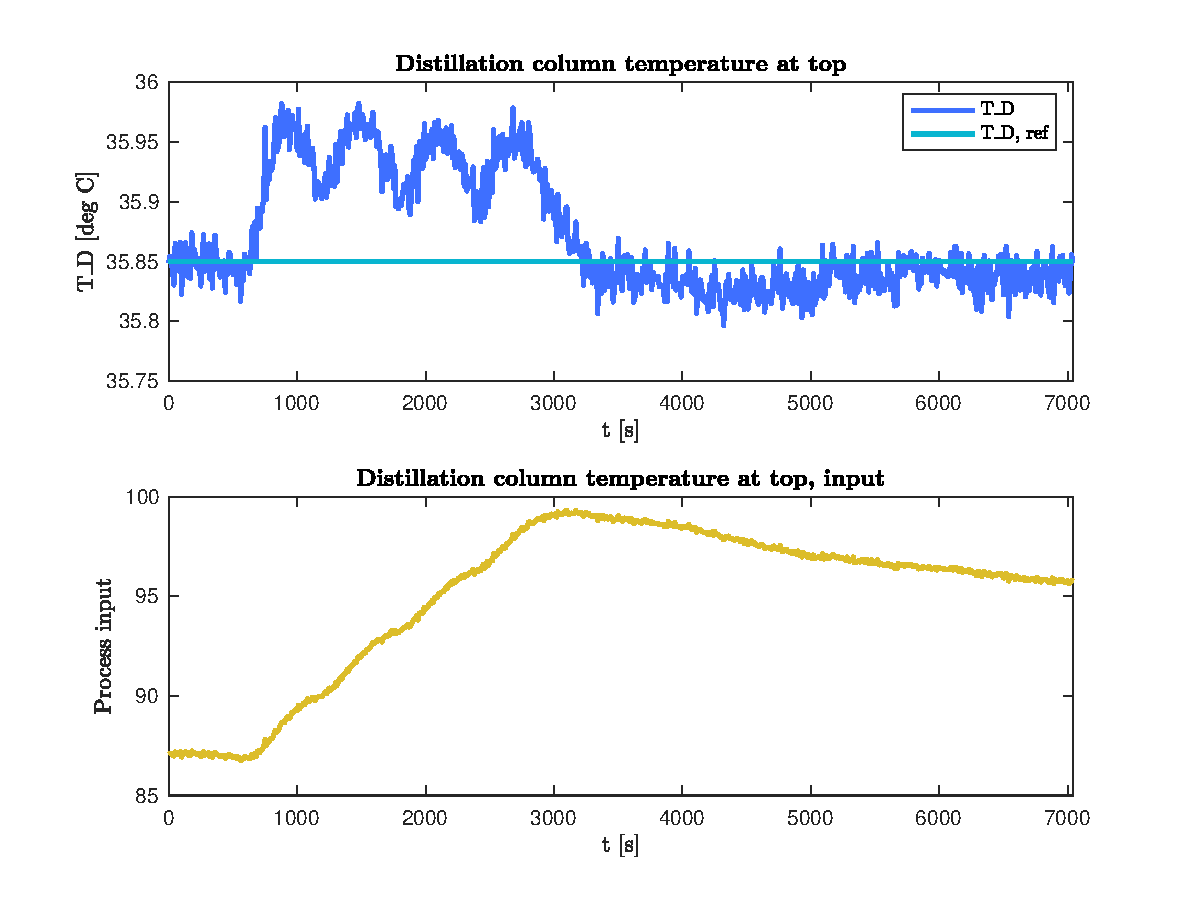
\includegraphics[width=0.8\textwidth]{../Systemanalyse/Log_Data_to_Matlab/Figurer/LV_tuning/T_D_closed_loop_with_stepwise_T_B_step.eps}
\caption{Response of controlled $T_D$ to stepwise step changes in $T_{B, \textrm{ref}}$}
\label{fig:TD_TB_cl_stepwise}

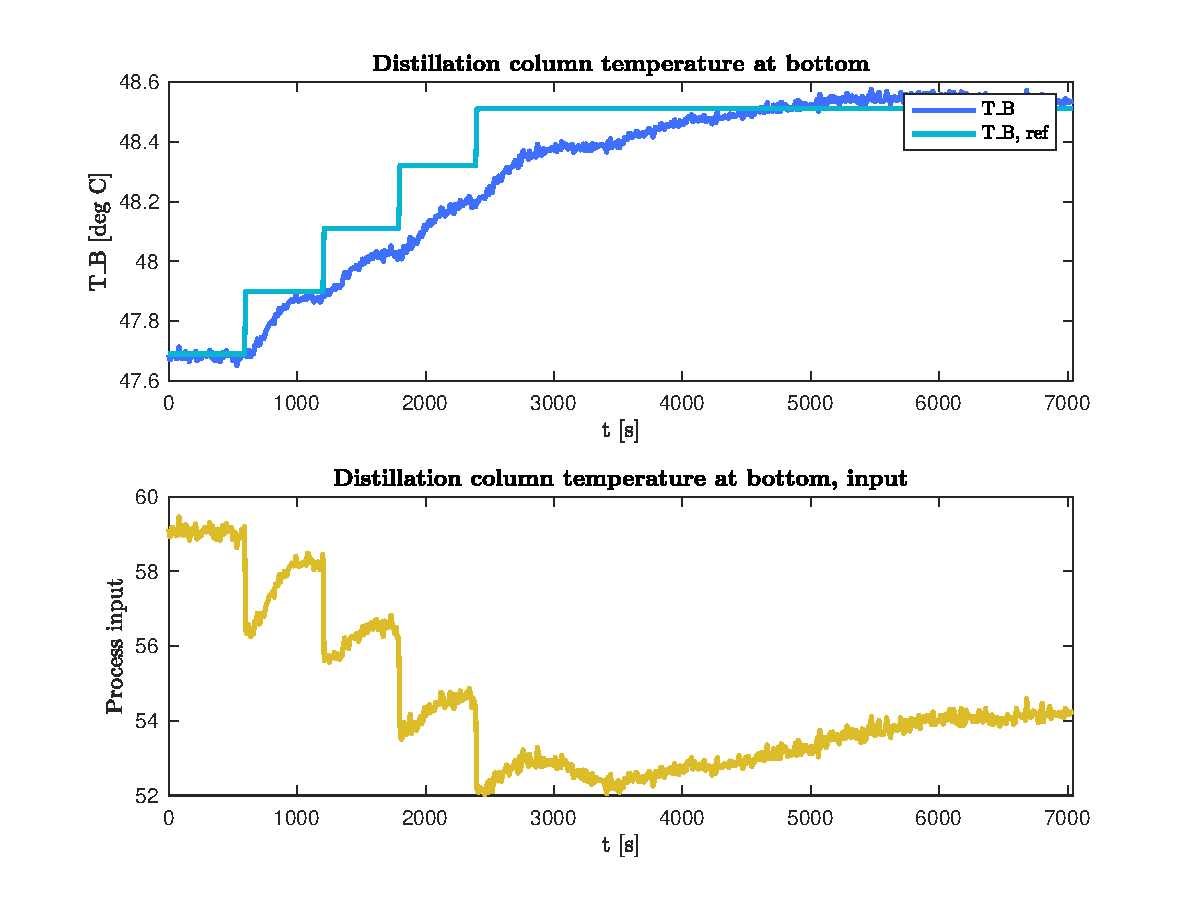
\includegraphics[width=0.8\textwidth]{../Systemanalyse/Log_Data_to_Matlab/Figurer/LV_tuning/T_B_closed_loop_with_stepwise_T_B_step.eps}
\caption{Response of controlled $T_B$ to stepwise step changes in $T_{B, \textrm{ref}}$}
\label{fig:TB_TB_cl_stepwise}
\end{figure}

\newpage
\section{Conclusion}
The control loops of the butane splitter was tuned to give stable responses, and for reasonable setpoints and setpoint changes, the temperature controllers should work satisfactory for the given requirements. The butane leaving Kårstø may safely be expected to adhere to specifications.

\newpage
\begin{thebibliography}{9}

\bibitem{oppgavetekst}
  Morten Hovd,
  \textit{TTK4210 Advanced Control of Industrial Processes, Assignment 6},
  2020.

\bibitem{skogestad}
  Sigurd Skogestad and Ian Postlethwaite,
  \textit{Multivariable Feedback Control},
  John Wiley \& Sons Ltd, Chichester,
  2nd edition,
  2005.
  
\bibitem{regtek}
  Jens G. Balchen, Trond Andresen and Bjarne A. Foss,
  \textit{Reguleringsteknikk},
  Institutt for Teknisk Kybernetikk, Trondheim,
  6th edition,
  2016.

\end{thebibliography}

\newpage
\appendix
\section{System identification experiments}
\subsection{Open-loop responses of manipulated variables}

\begin{figure}[p]
\centering
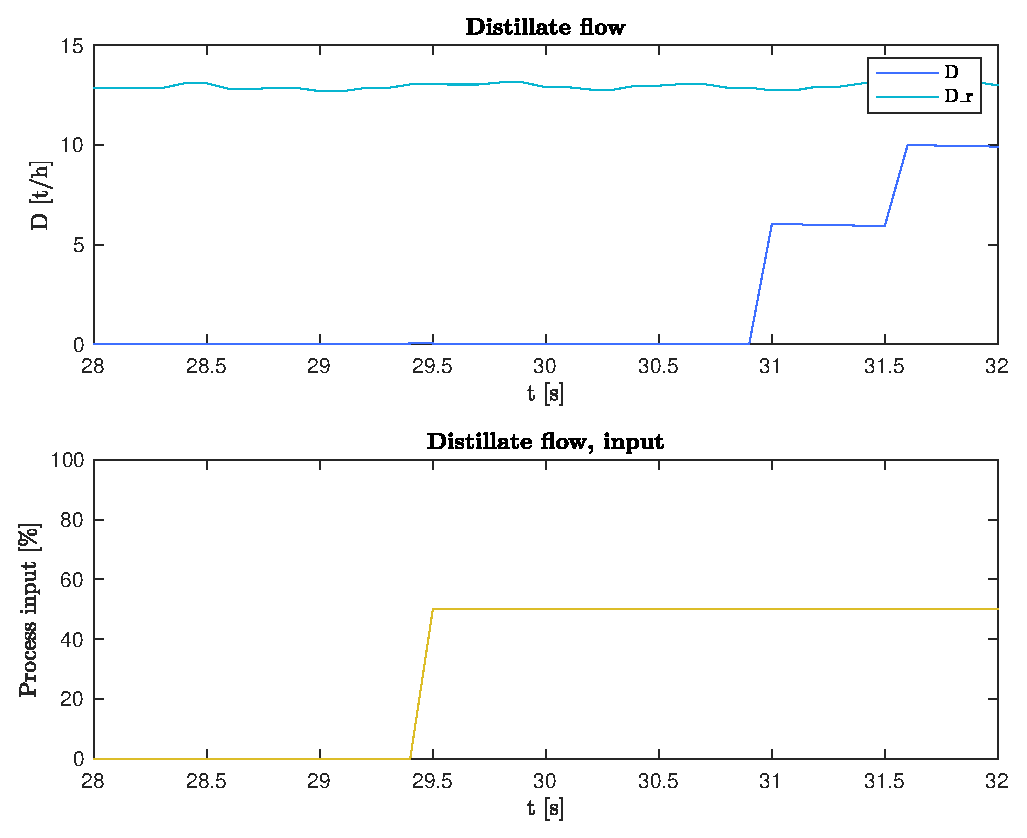
\includegraphics[width=0.8\textwidth]{../Systemanalyse/Log_Data_to_Matlab/Figurer/Stegeksperimenter/FC1005.eps}
\caption{Open-loop step response of $D$}
\label{fig:ol_step_FC1005}
\end{figure}

\begin{figure}[p]
\centering
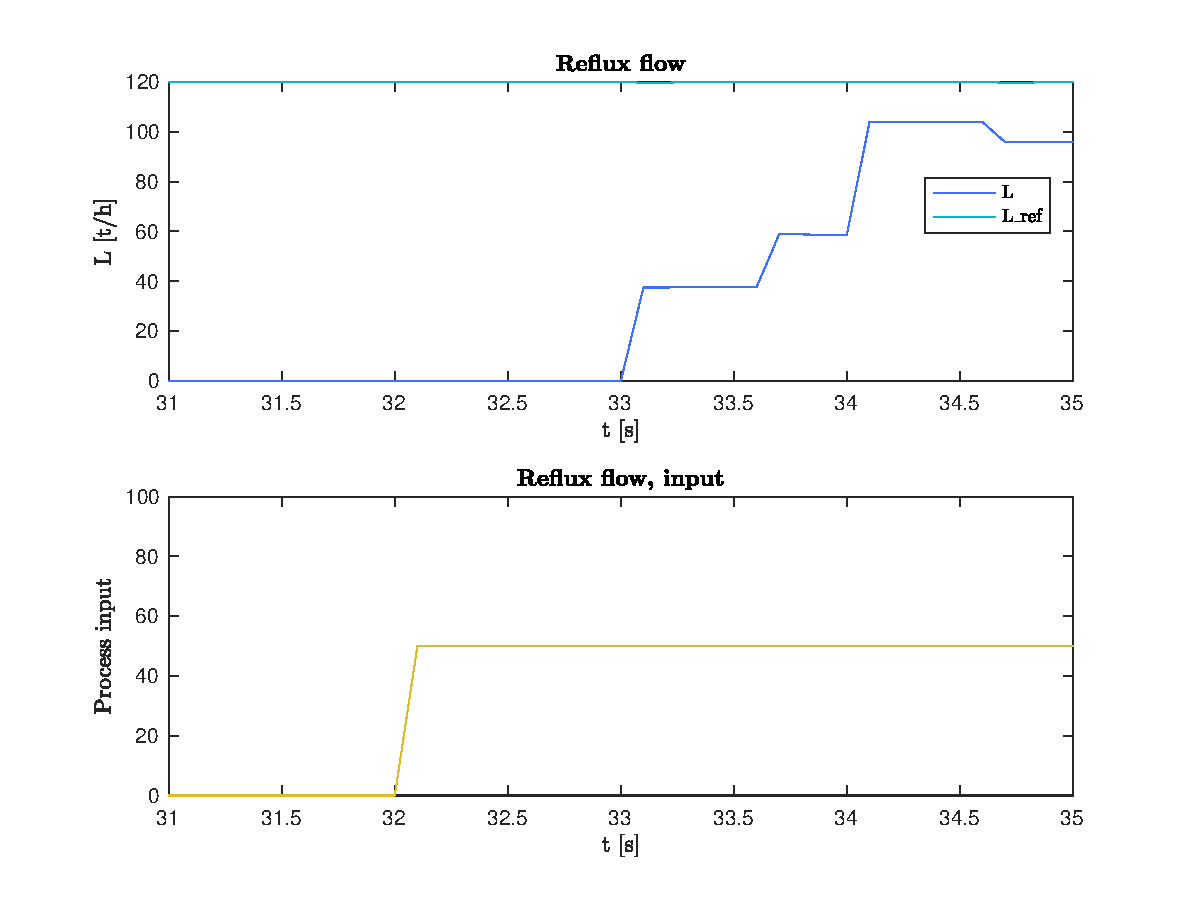
\includegraphics[width=0.8\textwidth]{../Systemanalyse/Log_Data_to_Matlab/Figurer/Stegeksperimenter/FC1015.eps}
\caption{Open-loop step response of $L$}
\label{fig:ol_step_FC1015}
\end{figure}

\begin{figure}[p]
\centering
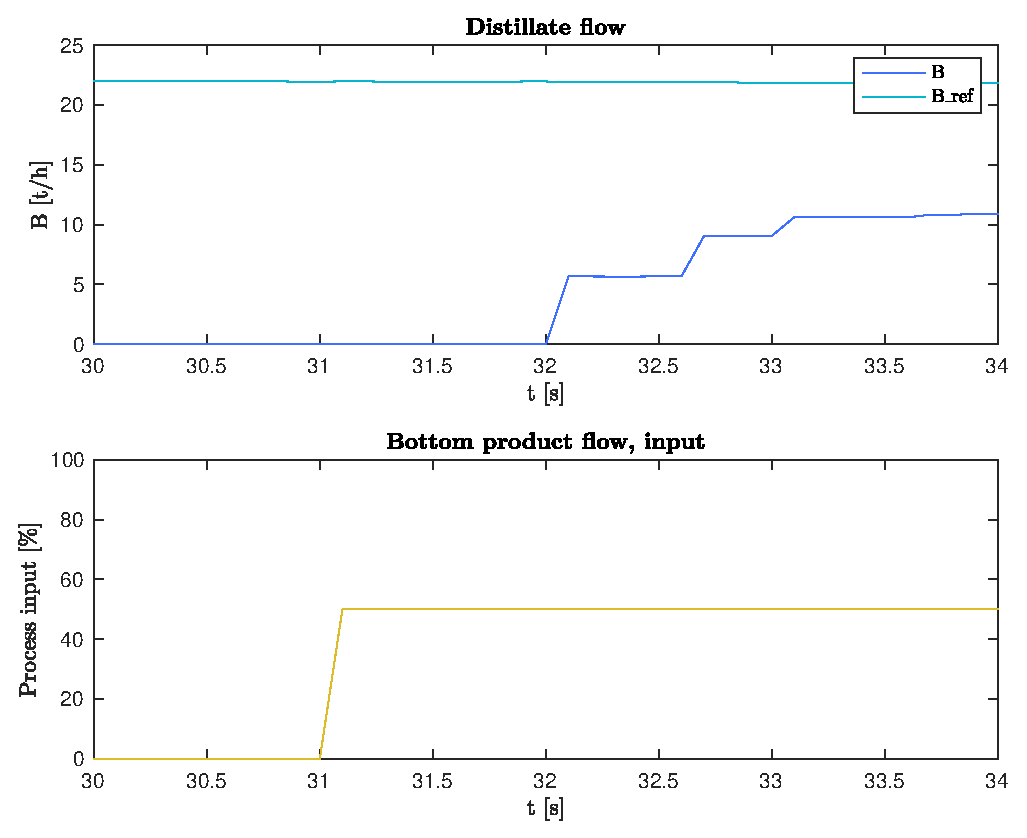
\includegraphics[width=0.8\textwidth]{../Systemanalyse/Log_Data_to_Matlab/Figurer/Stegeksperimenter/FC1019.eps}
\caption{Open-loop step response of $B$}
\label{fig:ol_step_FC1019}
\end{figure}

\begin{figure}[p]
\centering
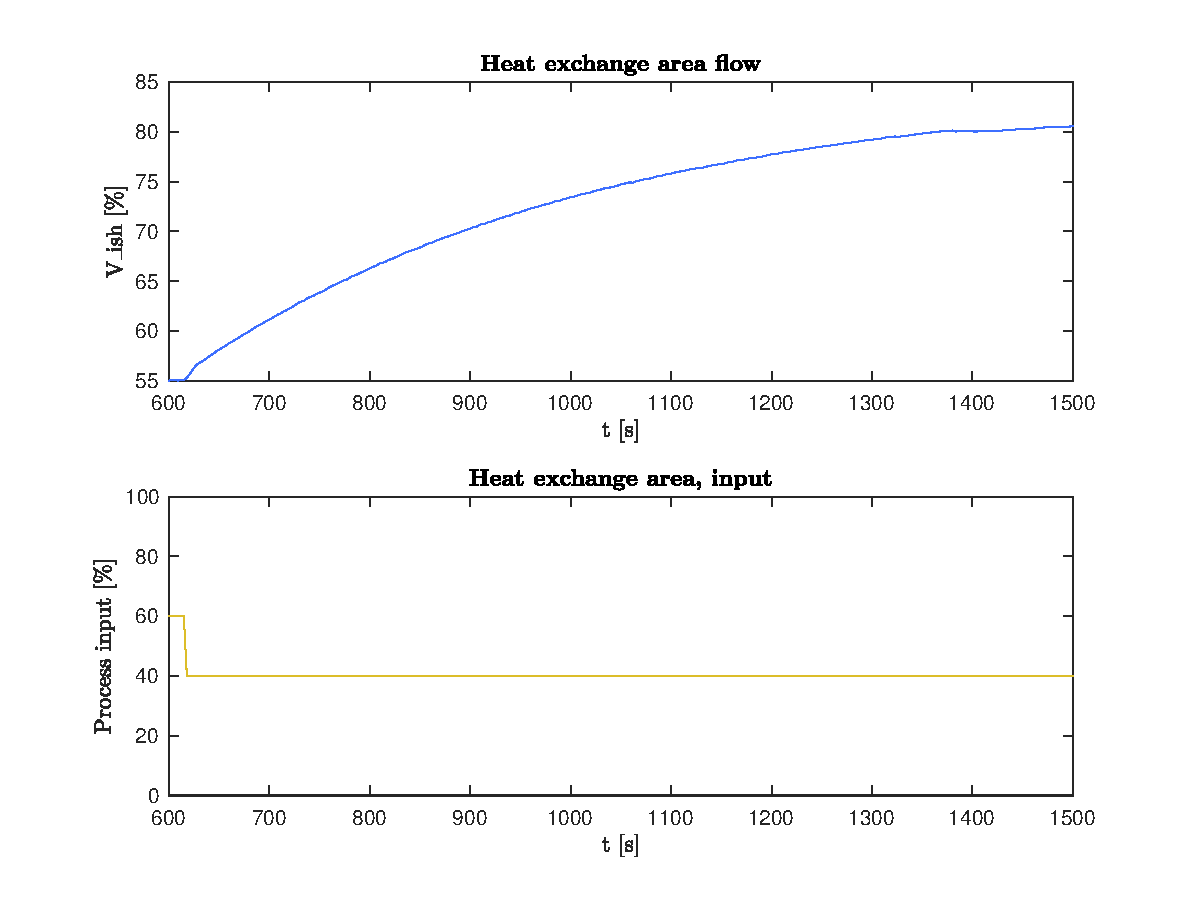
\includegraphics[width=0.8\textwidth]{../Systemanalyse/Log_Data_to_Matlab/Figurer/Stegeksperimenter/LC1028.eps}
\caption{Open-loop step response of heat exchanger area, related to $V$}
\label{fig:ol_step_LC1028}
\end{figure}

\begin{figure}[p]
\centering
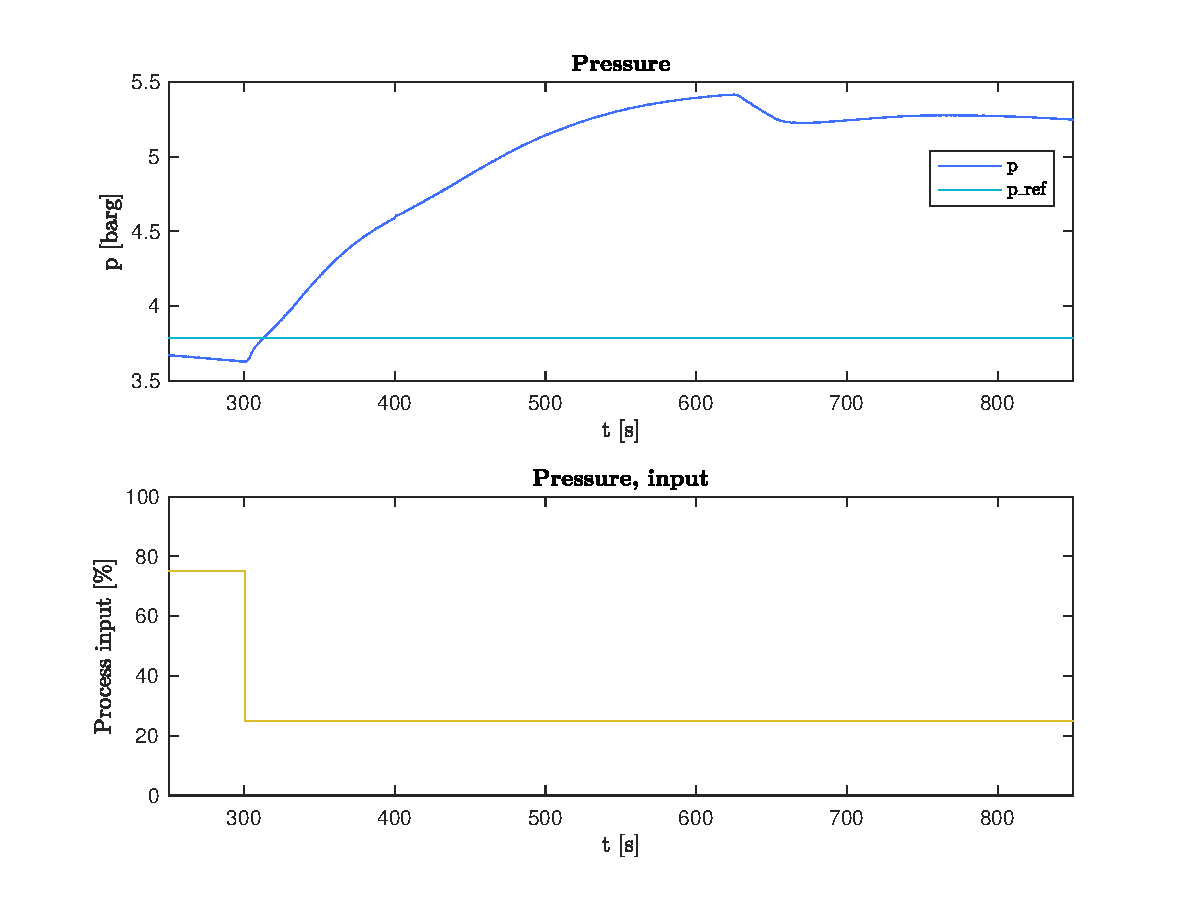
\includegraphics[width=0.8\textwidth]{../Systemanalyse/Log_Data_to_Matlab/Figurer/Stegeksperimenter/PC1024.eps}
\caption{Open-loop step response of $p$}
\label{fig:ol_step_PC1024}
\end{figure}

\subsection{System identification experiment for level control}

\begin{figure}[p]
\centering
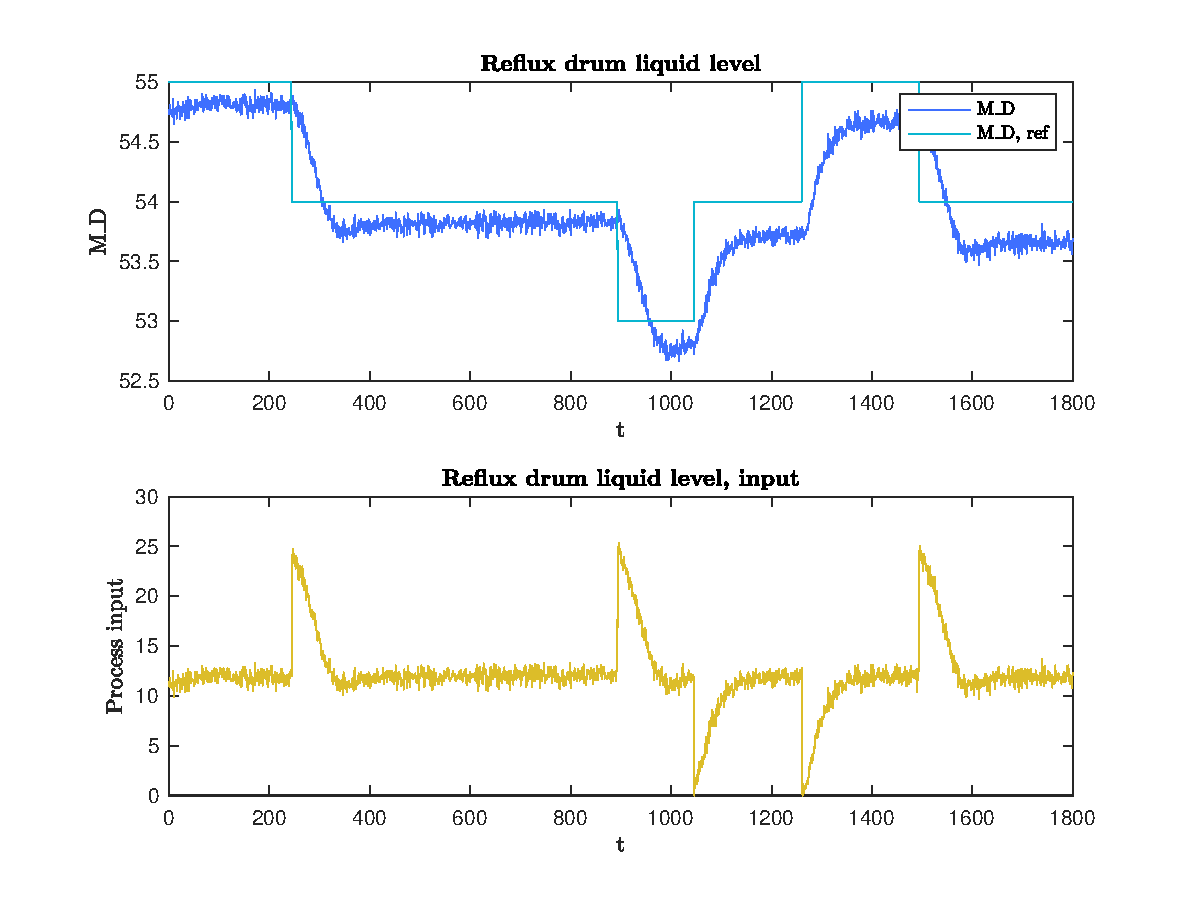
\includegraphics[width=0.8\textwidth]{../Systemanalyse/Log_Data_to_Matlab/Figurer/Identifisering/MD_eksperiment.eps}
\caption{System identification experiment for $M_D$ controller}
\label{fig:MD_experiment}

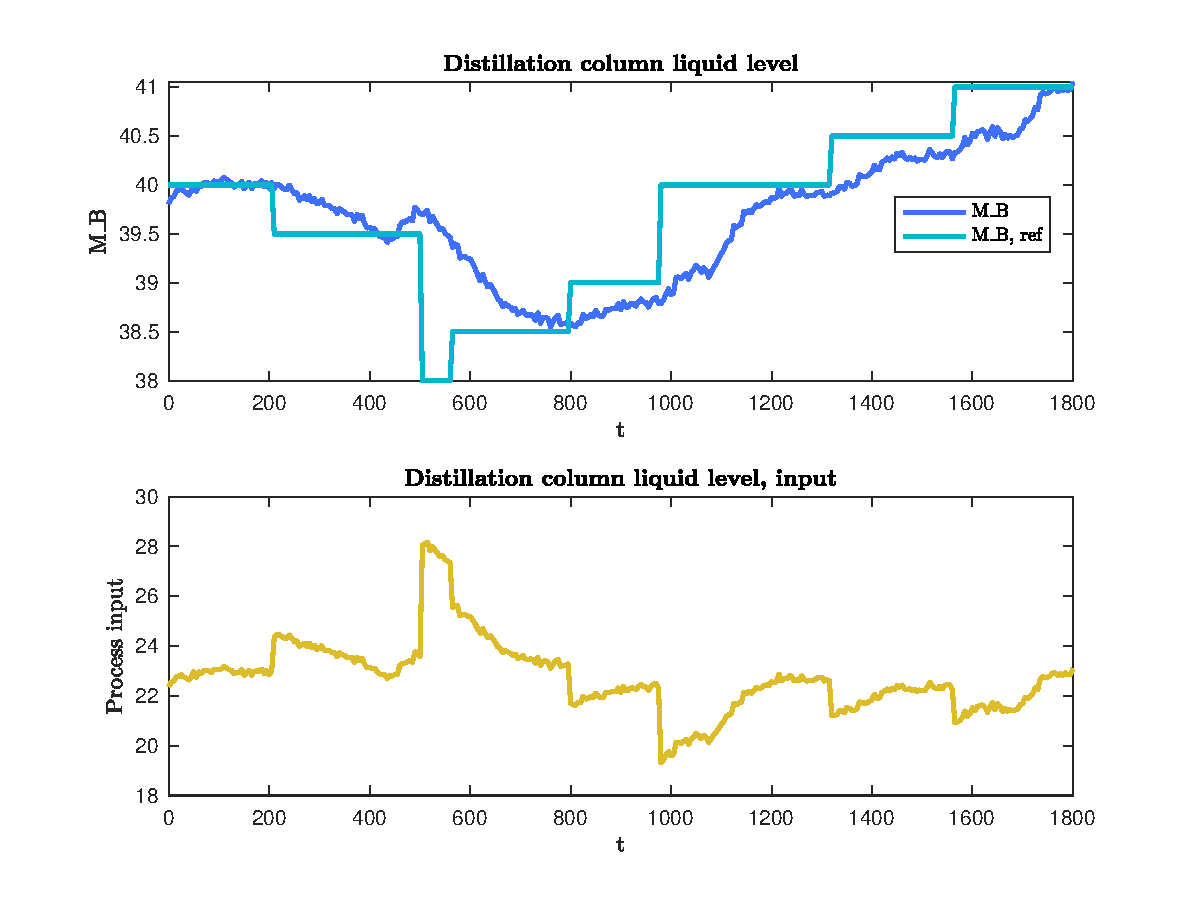
\includegraphics[width=0.8\textwidth]{../Systemanalyse/Log_Data_to_Matlab/Figurer/Identifisering/MB_eksperiment.eps}
\caption{System identification experiment for $M_B$ controller}
\label{fig:MB_experiment}
\end{figure}

\subsection{System identification experiment for composition (temperature) control}
\begin{figure}[p]
\centering
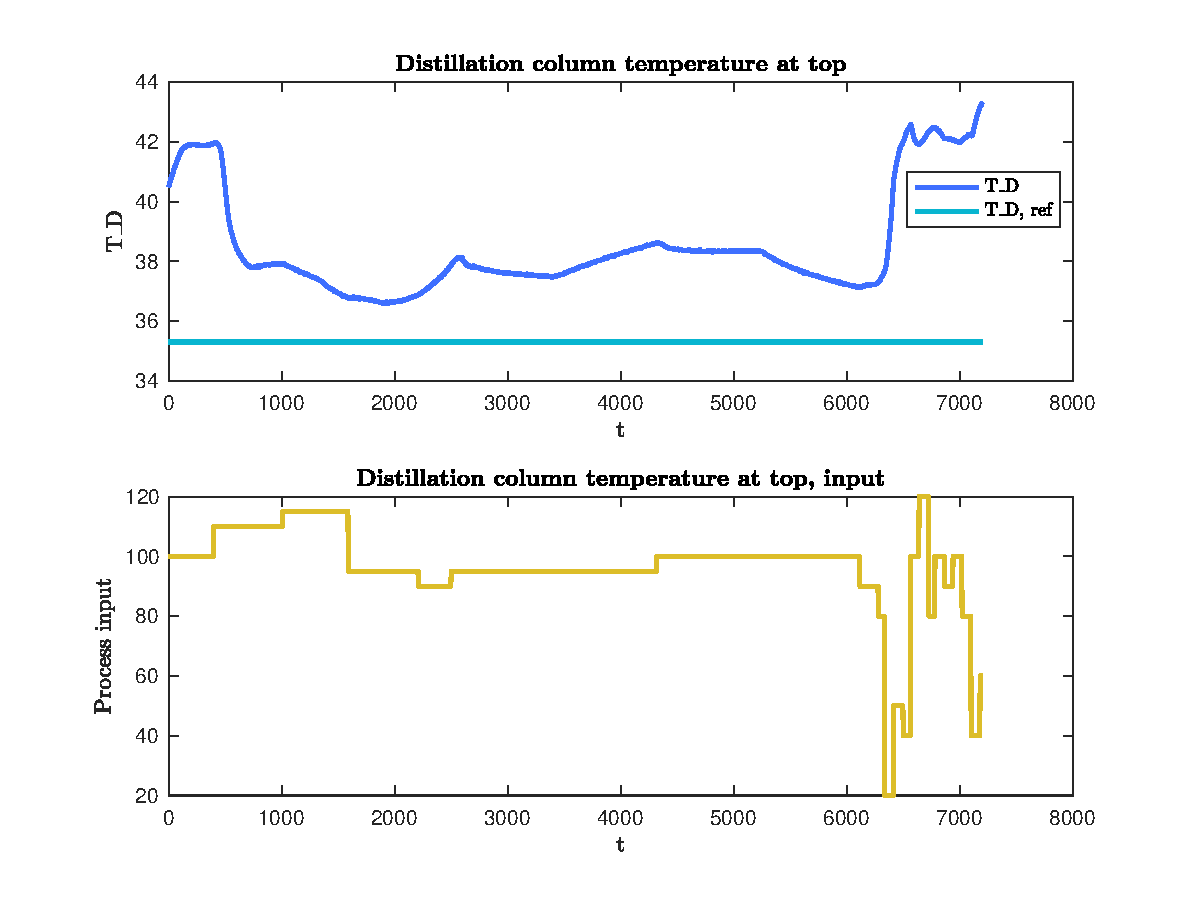
\includegraphics[width=0.8\textwidth]{../Systemanalyse/Log_Data_to_Matlab/Figurer/LV_identifisering/T_D_eksperiment.eps}
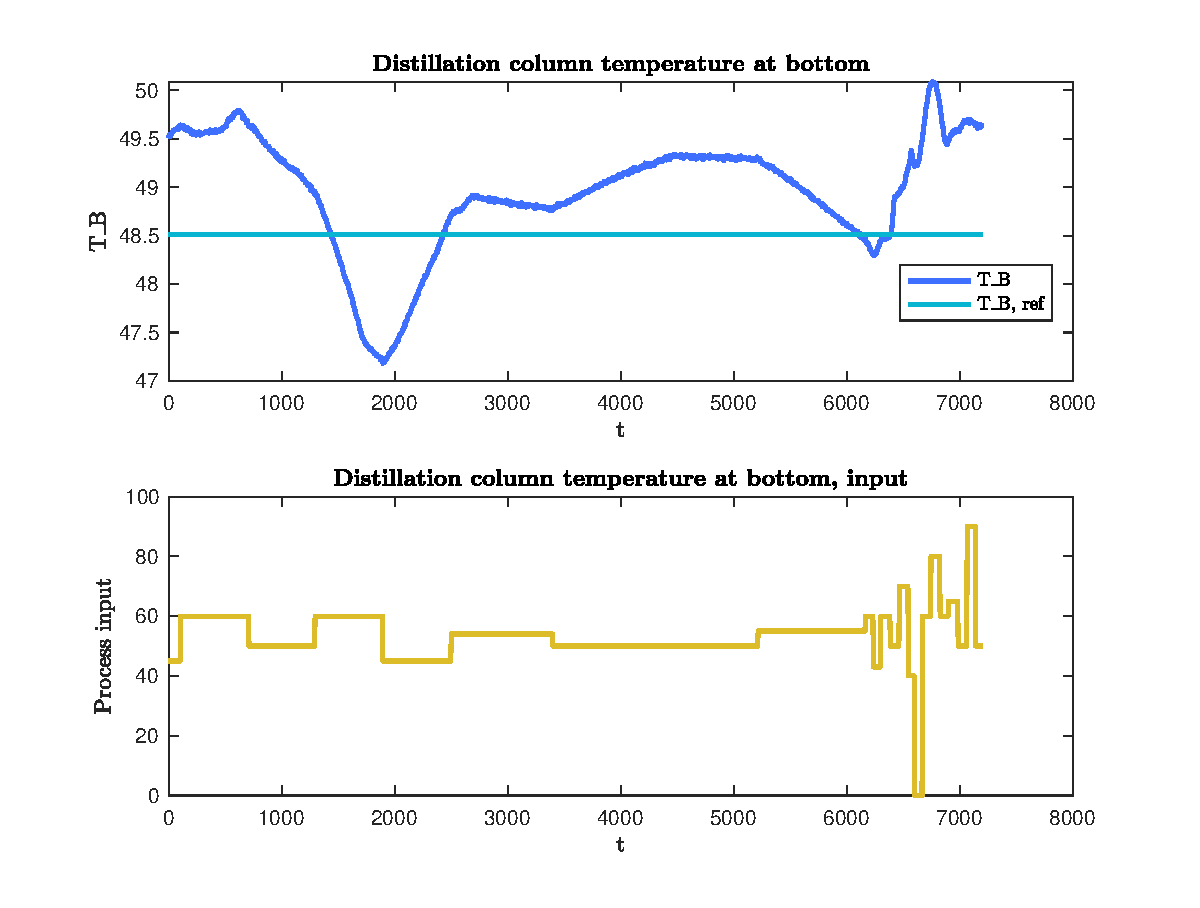
\includegraphics[width=0.8\textwidth]{../Systemanalyse/Log_Data_to_Matlab/Figurer/LV_identifisering/T_B_eksperiment.eps}
\caption{Response of $T_D$ and $T_B $ to step changes in $L$ and $V$}
\label{fig:LV_experiment}
\end{figure}

\end{document}
